
\chapter{A generic motif discovery algorithm}\label{chapter:gemoda}

\begin{comment}
\textbf{Motivation:}
Motif discovery in sequential data is a problem of great
interest and with many applications.  However, previous methods
have been unable to combine exhaustive search with
complex motif representations and are each
typically only applicable to a certain class of problems.

\textbf{Results:}
Here we present a GEneric MOtif DIscovery Algorithm
(Gemoda) for sequential data.  Gemoda can be applied to any
dataset with a sequential character, including both categorical
and real--valued data.  As we show,
Gemoda deterministically discovers motifs that are maximal
in composition and length.  As well, the algorithm allows any
choice of similarity metric for finding motifs.  Finally,
Gemoda's output motifs are representation--agnostic:
they can be represented using regular expressions,
position weight matrices, or any number of other models for any
type of sequential data.
We demonstrate a number
of applications of the algorithm, including the discovery
of motifs in amino acids sequences, a new solution to the
(l,d)--motif problem in DNA sequences, and the discovery of
conserved protein sub--structures.

\textbf{Availability:}
Gemoda is freely available at \url{http://web.mit.edu/bamel/gemoda}.

\textbf{Contact:}
gregstep@mit.edu

\textbf{Supplementary Information:}
Available at \url{http://web.mit.edu/bamel/gemoda}.
\end{comment}


\section{Introduction}
In the previous chapter, I described the use of regular grammars for
modeling the primary sequences of antimicrobial peptides.  In that
work, I showed that our specific approach to the design of novel
AmPs yielded peptides with strong antimicrobial activity.  However,
recall that, in order to achieve specificity with some degree of
sensitivity, the grammars had to be split into tiled 10 amino acid
windows for increased sensitivity and then compared against a
database of non--AmP sequences in order to increase specificity by
throwing out uninformative grammars.  This is because, as discussed
in Chapter~\vref{chapter:intro}, regular grammars are inherently
more ``coarse grained'' then other models such as position weight
matrices.  Thus, to design AmPs, we had to use large sets of
redundant, overlapping regular grammars.  In such situations, the
underlying sequence information might be better modeled by a
position weight matrix or many other kinds of models.

In this chapter, I present a GEneric MOtif DIscovery Algorithm
(Gemoda) for sequential data.  Gemoda is a motif discovery tool very
similar to Teiresias; however, Gemoda's output motifs are
representation--agnostic: they can be represented using regular
expressions, position weight matrices, or any number of other
models. In addition, Gemoda can be applied to any dataset with a
sequential character, including both categorical data such as
protein and amino acid sequences, and real--valued data such as the
price of a stock as a function of time. As I show in the following
sections, Gemoda deterministically discovers motifs that are maximal
in composition and length.  As well, the algorithm allows any choice
of similarity metric for finding motifs. I demonstrate a number of
applications of the algorithm, including the discovery of motifs in
amino acids sequences, a new solution to the (l,d)--motif problem in
DNA sequences, and the discovery of conserved protein
sub--structures.

The research described in this chapter is drawn
largely from two publications:
    \begin{itemize}
    \item M. Styczynski, K. Jensen, I. Rigoutsos, \&
    G. Stephanopoulos. ``An extension and novel solution to the
    (l,d)-motif challenge problem.'' 
    \emph{Genome Inform Ser Workshop Genome Inform.} 2004;15(2):63--71; and

    \item K. Jensen, M. Styczynski, I. Rigoutsos, \& G. Stephanopoulos.
    ``A generic motif discovery algorithm for sequential data,''
    \emph{Bioinformatics} 22:21-28 (2006).
    \end{itemize}
    Throughout this
    chapter, the use of the pronoun ``we'' refers to the
    authors of these  manuscripts.

\section{Motivation}

As discussed in Chapter~\vref{chapter:intro}, motif discovery
encompasses a wide variety of methods used to find recurrent trends
in data. In bioinformatics, the two predominant applications of
motif discovery are sequence analysis and microarray data analysis.
Less common applications include discovering structural motifs in
proteins and RNA~\citep{holm1992database,murthy2003rnabase}.
\index{protein!structure}

Motif discovery in sequence analysis typically involves the
discovery of binding sites, conserved domains, or otherwise
discriminatory subsequences. There are many publicly--available
tools, a large number of which are listed in
Section~\vref{section:tools}, each of which is quite adept at
addressing a specific subclass of motif discovery problems. Some of
the commonly--used tools for motif discovery in nucleotide and amino
acid sequences include MEME~\citep{bailey1994fitting}, Gibbs
sampling~\citep{lawrence1993detecting},
Consensus~\citep{hertz1999identifying}, Block
Maker~\citep{henikoff1995automated},
Pratt~\citep{jonassen1995finding}, and
Teiresias~\citep{rigoutsos1998combinatorial}. Newer, less-widely
used tools include Projection~\citep{buhler2001finding},
MultiProfiler~\citep{keich2002finding},
MITRA~\citep{eskin2002finding}, and
ProfileBranching~\citep{price2003finding}.  This list is not
intended to be exhaustive; however, it is indicative of the wealth
of options available for solving such problems (see also
Tables~\ref{table:regexMD} \&~\ref{table:pwmMD} in Chapter~\ref{chapter:intro} on pages~\pageref{table:regexMD} \&~\pageref{table:pwmMD}, respectively).

All of the existing motif discovery tools for nucleotide and amino
acid sequences can be classified on a spectrum ranging from
exhaustive tools using simple motif representations to
non--exhaustive tools using more complex representations.  The
majority of the tools can be found at the extreme ends of the
spectrum, with tools that exhaustively enumerate regular expressions
(or single consensus sequences) at one end and probabilistic tools,
based on position weight matrices (PWMs), at the other. This
partitioning of tools is due to a computational trade--off: more
descriptive motif representations such as PWMs frequently make
exhaustive searches computationally infeasible.


One of the primary motivation for this work is the modeling of
cis--regulatory sequences. We found that regular expressions are
poor representations of binding sites and that, instead, these were
better captured with PWMs.  From a biological perspective, this
makes more sense --- the $k_D$ of binding between the trans and cis
factors are probabilistic, not deterministic.  Thus, in order to
model these sites using regular grammars or regular expressions, one
must, in general, use combinations of patterns in an effort to piece
together the information that would be contained within a PWM from
many regular expressions.

Consider the following example.  The LexA regulon consists of 9 gene
sequence that are regulated by a single protein trans factor.  The
binding site of this trans factor is found in 8 of these sequences.
Using the Teiresias motif discovery tool, with parameters $L=10,
W=20, K=5$ (see Section~\vref{section:teiresias}) returns the
following patterns\\
    {
    \begin{center}
    \ttfamily
        \begin{singlespace}
    \begin{tabular}{ccl}
        5 & 4 & CTGTATAT.....CAG 0 355 0 376 4 298 6 326 7 363 \\
        5 & 5 & CTGTAT....A..CAG 0 376 1 322 4 298 6 326 7 363 \\
        5 & 5 & ACTGTA.....A..CAG 0 375 1 321 3 358 4 297 7 362 \\
        5 & 5 & CTGTA.AT..A..CAG 0 376 3 359 4 298 6 326 7 363\\
        6 & 5 & CTGTA.AT.....CAG 0 355 0 376 3 359 4 298 6 326 7 363\\
        5 & 5 & ACTGT.T....A..CAG 0 375 1 321 4 297 5 307 7 362\\
        5 & 5 & ACTGT...T..A..CAG 0 375 3 358 4 297 5 307 7 362\\
        5 & 5 & CTGT.T.T..A..CAG 0 376 4 298 5 308 6 326 7 363
    \end{tabular}
        \end{singlespace}

    \end{center}
    }
where the above grammars have been left and the native output form
of Teiresias.  The numbers on the right hand side indicate the
offset list for each grammar. So, collectively, these patterns hit 7
of the 8 sequences; however, none of the patterns individually hits
more than 5 sequences. Basically, this is because regular
expressions don't capture such sites well.


And this chapter, I described Gemoda: a motif discovery tool that
has many of the strengths of Teiresias, but can find motifs that are
best represented as PWMs.  The details of Gemoda are discussed in
the later sections of this chapter.  But here, for motivation,
consider the following output from the Gemoda all over them.  If a
user tells Gemoda to find all patterns in the LexA sequences such
that, on a pairwise basis, each window of 20 nucleotides in each
instance contains at least 10 nucleotides in common to each other
instance, and the pattern occurs in at least 8 sequences; Gemoda
returns
only a single pattern: \\
    {
    \begin{center}
    \ttfamily
    \begin{singlespace}
    \begin{tabular}{ccl}
       0  353 &TGCTGTATATACTCACAGCA \\
       0  374 &AACTGTATATACACCCAGGG \\
       1  320 &TACTGTATGAGCATACAGTA \\
       2  230 &ACCTGAATGAATATACAGTA \\
       3  357 &TACTGTACATCCATACAGTA \\
       4  296 &TACTGTATATTCATTCAGGT \\
       5  306 &AACTGTTTTTTTATCCAGTA \\
       6  324 &ATCTGTATATATACCCAGCT \\
       7  361 &TACTGTATATAAAAACAGTA \\
    \end{tabular}
    \end{singlespace}
    \end{center}
    }
where, instead of one pattern per line, each line represents one of
the offsets and the numbers on the left--hand side are,
collectively, the offset list. Notice that here, only a handful of
the positions within the pattern are fully conserved . However, most
of the positions have ``preferences.'' For example, the seventh
position is mostly A\@. This pattern can be expressed as a PWM, has
in Figure~\vref{fig:lexaLogo}, thus preserving these preferences in
the matrix probabilities. Notably, this pattern is exactly the
experimentally determined motif.

            \begin{figure}[ptb]
        A)
            \begin{center}
            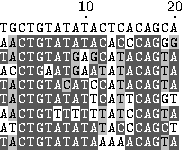
\includegraphics[width=0.4\textwidth]{Body/Images-chap3/lexa.pdf}
            \end{center}
        \bigskip
        B)
            \begin{center}
            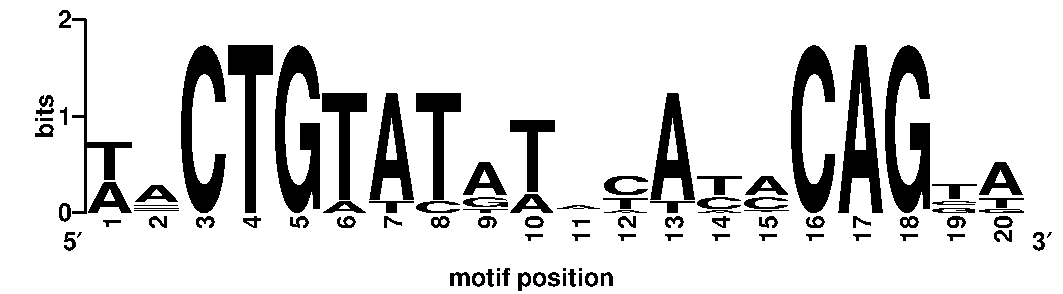
\includegraphics[width=\textwidth]{Body/Images-chap3/lexa1.pdf}
            \end{center}
        \bigskip
            C)
            \begin{center}
        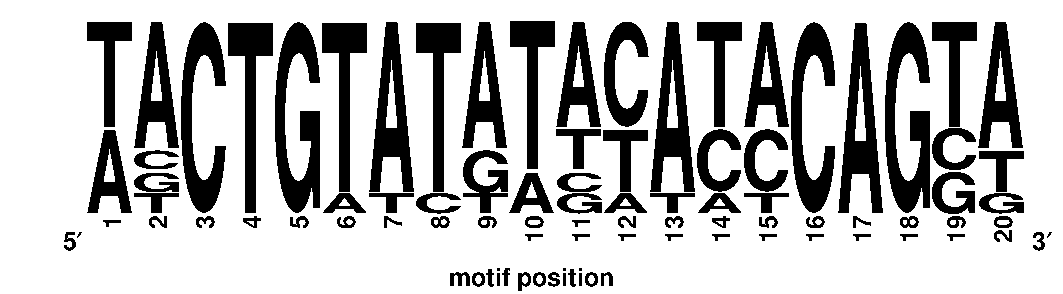
\includegraphics[width=\textwidth]{Body/Images-chap3/lexa2.pdf}
            \end{center}
            \caption[Alignment representing the LexA cis--regulatory binding site]{
                Alignment representing the LexA cis--regulatory binding site.
                Part A) of the figure shows the aligned sequences
                colored to indicate the degree of conservation.
                Part B) of the figure shows a sequence logo
                representing the information content of a PWM
                computed from the alignment of the motif instances.
                Part C) of the figure shows a sequence logo, wherein
                the height of each letter is proportional to its
                frequency, rather than to the information content it
                in codes as is the case in part B).
            }
            \label{fig:lexaLogo}
            \end{figure}


Depending on the task at hand, a specific type of motif discovery
tool may be more useful than others.  For example, the PWM--based
tools excel at finding \textit{cis}--regulatory binding
elements~\citep{tompa2005assessing}, whereas the regular
expression--based tools are well--suited to finding conserved
domains in large protein families~\citep{rigoutsos1999dictionary}.
Generally, it can be difficult to know \textit{a priori} which motif
discovery tool will be right.  Accordingly, there is an unmet need
for motif discovery tools that can use a variety of motif models.


\section{Algorithm}

    Gemoda was designed to meet the demand for complex
    motif representations, like PWMs, while still
    being exhaustive.  The philosophical underpinnings
    of the Gemoda algorithm can be traced back to
    Teiresias~\citep{rigoutsos1998combinatorial};
    Winnower~\citep{pevzner2000combinatorial}; the
    algorithm by~\citep{mancheron2003pattern}; and
    a variety of algorithms for association
    mining~\citep{zaki2000scalable,zaki1998theoretical}.
    In particular, Gemoda shares some of its logical steps
    with the Teiresias algorithm while incorporating a
    more flexible definition of ``similarity'' and allowing
    motif representations other than regular expressions.

The principle difference between Teiresias and most frequent itemset
mining algorithms is that Teiresias acts on categorical sequential
 data, usually biosequences or integers.  Most frequent itemset mining tools use market
basket data sets, for example, a collection of products that a
customer bought.  Patterns in market basket data can be used to
predict what other products a customer might buy (this is how
Amazon.com works). The difference between categorical sequential
data and market basket data (both are stochastic in that they
consist of discrete values sampled from some real space) is that the
former is ordered, whereas the latter is an unordered set.  For
similarly sized datasets, this makes sequential pattern discovery
much easier. However, typically sequential datasets, such as
biosequences or time--series stock data, are much larger.  For
example, a person may only purchase a few products from Amazon;
however, gene sequences can consist of may thousands of characters.

    Gemoda's design goals can be summarized
    as follows: \emph{exhaustive discovery} of all
    \emph{maximal motifs} in a way that allows
    flexibility in \emph{motif representation},
    incorporation of a variety of
    \emph{similarity metrics}, and the ability to handle
    diverse \emph{sequential
    data types}.  Each point of emphasis can be explained
    as follows:
        \begin{itemize}

        \item\textbf{Exhaustive discovery:} Gemoda's combinatorial
            nature provides an algorithmic
            guarantee that all motifs meeting
            certain criteria are deterministically
            discovered.

        \item\textbf{Maximal motifs:} Gemoda
            returns only motifs that are maximal
            in both length and composition with respect
            to the similarity and clustering functions.


        \item\textbf{Motif representation:}  The motifs
            discovered by Gemoda are reported as
            short multiple
            sequence alignments (in the case of
            motif discovery in nucleotide and amino
            acid sequences) and can be
            modeled using regular expressions,
            PWMs/PSSMs, Markov models, or any
            other representation.

        \item\textbf{Similarity metrics:} Any criterion, ranging
            from sequence alignment scores to
            geometric functions, may be used to
            compare sequences.

        \item\textbf{Sequential data types:} The
            nature of Gemoda's computations is not
            unique to any specific type of data,
            and thus can be used on any data with
            a sequential character --- that is,
            data in which there is a natural
            left--to--right order, such as a
            sequence of nucleotides or amino acids.
            In the most general sense, sequential data
            also include real--valued series data,
            such as a stock price or the ordered
            $(x,y,z)$ triplets of an alpha--carbon
            trace in a protein structure.



        \end{itemize}

    The algorithm has three distinct phases:
    comparison, clustering, and convolution.  During the
    comparison phase, short overlapping windows in the data
    set are compared.  During clustering, these windows
    are grouped together to form elementary motifs.
    Finally, during convolution, these motifs
    are ``stitched'' together to form maximal motifs (see
    Figure~\vref{fig:gemoda}).  In the following sections,
    we give some brief definitions and nomenclature,
    then describe each of the algorithm's three phases
    in detail.  Finally, we illustrate a few applications
    of Gemoda.


    \begin{sidewaysfigure}[ptb]
        \centering
        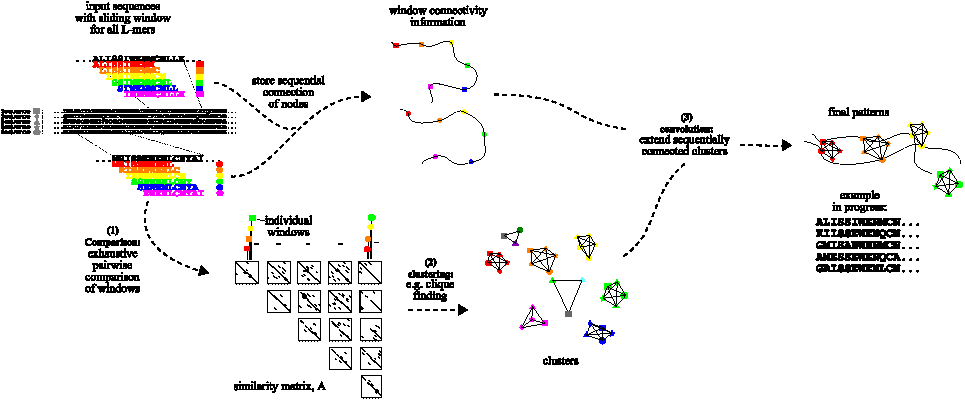
\includegraphics[width=\textheight]{Body/Images-chap3/gemoda_fig5.pdf}
        \caption[A sketch showing the flow of the Gemoda algorithm
            for an example input set of protein sequences.]{A sketch showing the flow of the Gemoda algorithm
            for an example input set of protein sequences.
            The various colors in the input sequences are used
            to indicate the sequential ordering of the $L$--residue
            windows.  The various shapes are used to indicate
            a particular window's sequence of origin.  (1) In the
            comparison stage, each window is compared to each
            other window on a pair--wise basis.  Here we show
            the similarity matrix, $A$, where the values in the
            matrix have been thresholded.  Those pairs of windows
            in $A$ that have a similarity score above the threshold
            are colored black.  Note that the graph looks very
            similar to a standard dot plot.  (2) In the clustering
            phase, groups of windows are clustered together.
            Here, we show the clusters as cliques, or maximal
            fully--connected subgraphs in the thresholded matrix
            $A$.  (3) Finally, these clustered are ``stitched'' together
            in the convolution phase using the sequential ordering
            of the windows to reveal the maximal motifs.
            A similar process
            applies for any kind of sequential data analyzed by
            Gemoda.
        }\label{fig:gemoda}
    \end{sidewaysfigure}

    \subsection{Preliminary definitions and nomenclature}

    The input to Gemoda is a set of sequences of
    data points $S=\braces{s_1,s_2,\ldots,s_n}$, where
    sequence $s_i$ has length $W_i$.  So, for example,
    the $\ith{j}$ member of the $\ith{i}$ sequence
    is denoted by $s_{i,j}$.  Each $s_{i,j}$ is a
    primitive, or atomic unit, for the data that is
    being analyzed.  For time--series data, $s_{i,j}$
    may be a point sampled from $\realNums^{K}$ (with
    $K$ arbitrary), whereas for a DNA sequence it would
    be one of the characters $\{\texttt{A,T,G,C}\}$.

        To demonstrate this notation and how he can be used to
        represent real--valued sequential data, rather biosequences
        consider the following example.
        Say we have two small peptides and we are interested in their
        structural properties.  For each amino acid, we have a two--dimensional
        feature vector.  The first feature is the hydrophobicity index~\cite{argos1982structural}
        and the second is the size of the amino acid: 1 if it is over the
        50$^{th}$ percentile and 0 otherwise.  The two peptides are \texttt{AIKDWR}
        and \texttt{DIHV}\@.  Our two sequences are then
        \begin{eqnarray*}
            \text{seq--0} & = & \begin{pmatrix}
                        0.61 & 2.22 & 1.15 & 0.46 & 2.65 & 0.60\\
                        0 & 1 & 1 & 0 & 1 & 1
                    \end{pmatrix} \\
            \text{seq--1} & = & \begin{pmatrix}
                        0.46 & 2.22 & 0.61 & 1.32 \\
                        0 & 1 & 1 & 0
                    \end{pmatrix},
        \end{eqnarray*}
        such that
        \begin{eqnarray*}
            s_{0,0,0} & = & 0.61 \\
            s_{1,0,0} & = & 0.46 \\
            s_{1,1,1} & = & 1 \\
            s_{0,3,1} & = & 0 \\
            s_{1,2,0} & = & 0.61,
        \end{eqnarray*}
        and so on.

    Typically, one seeks motifs
    of a minimal, domain--dependent length.
    We denote this minimum length by $L$
    (similar to Teiresias)
    and we define a matrix $A$ of size
    $N\times N$, where $N = \sum_{i=1}^{n}(W_i-L+1)$.
    That is, $A$ is a matrix with one row and one column for each
    window of size $L$ in our entire sequence set.
    For example, the $10^{th}$ window of size $L$ in the $5^{th}$
    sequence would be expressed as $s_{5,10:10+L-1}$,
    where ``$10:10+L-1$'' denotes ``position $10$
    through position $10+L-1$, inclusive.''  To keep
    track of which window corresponds to which index
    in $A$, we define the one--to--one function
    $\mathscr{M}(s_{i,j:j+L-1})\mapsto q \in [1,N]$.
    (For simplicity, we define
    $(s_{i,j}+1)$ to be $s_{i,j+1}$, unless $s_{i,j+1}$
    does not exist, in which case $(s_{i,j}+1)$
    is undefined.)  Similarly, $\mathscr{M}^{-1}(q)
    \mapsto (s_{i,j:j+L-1})$ such that $i\in[1,n]$
    and $j \in [1,W_i-L+1]$.

    We also define a similarity function
    $\mathscr{S}(s_{i,j:j+L-1}, s_{q,z:z+L-1})$,
    that takes as arguments two
    arbitrary windows and returns a real--valued number
    indicating the level of similarity between the two
    windows.  In the most simple case, $\mathscr{S}$
    may use the identity matrix to count how
    many DNA bases two windows have in common;
    for real--valued data, the function may return
    the sum--of--squares error between two windows
    or any other measure of similarity.


    We define a motif $p$ as a data structure
    with two features: a width $\mathscr{W}(p)$
    and a list of locations in the data where the
    motif occurs, $\mathscr{L}(p)$.  A motif has the
    property that the locations in $\mathscr{L}(p)$
    meet some predefined clustering requirements
    (discussed below) based on the similarity function
    $\mathscr{S}$ for each window of length $L$ within
    the motif.  The support of a motif is equal to
    the number of its occurrences (or, equivalently, ``instances'' or ``embeddings''),
    $\vert \mathscr{L}(p) \vert$.

    We say a maximal motif is a motif which has the following properties:
        \begin{enumerate}
        \item   The motif's width cannot be extended in
            either direction (left or right)
            without producing a motif with
            fewer embeddings (i.e., without
            $\vert \mathscr{L}(p) \vert$
            decreasing); and

        \item   The motif is not missing any instances,
            i.e.\ $\mathscr{L}(p)$ includes the locations
            of all instances of the motif.

        \end{enumerate}
    These two criteria can be summarized qualitatively by stating that a maximal
    motif is not ``missing'' any locations and is as wide as possible, and
    thus it is as specific and sensitive as possible.

    Given these explanations and definitions, we can now detail
    the computations involved in each phase of the Gemoda algorithm.
    A simple natural--language example illustrating how each phase
    proceeds is included in the supplementary materials.

    \subsection{Comparison phase}
    In the comparison phase of the Gemoda algorithm,
    the sequences are divided into overlapping windows
    of size $L$ which are then compared to each other
    in a pairwise manner to produce a similarity
    matrix, $A$ (see Figure~\vref{fig:gemoda}).
    Formally, $A_{i,j}$ is equal to
    $\mathscr{S}(\mathscr{M}^{-1}(i),\mathscr{M}^{-1}(j))
    = \mathscr{S}(s_{i,j:j+L-1}, s_{q,z:z+L-1})$.

    $A$ is then, quite simply, a similarity matrix
    for all $N$ windows based on the similarity
    function $\mathscr{S}$.
    In most cases, $\mathscr{S}$
    is commutative (and the $A$ matrix is symmetric);
    however, this is not a requirement.

        Consider the following example.
        Say we have two DNA sequences --- seq--0 = \texttt{AATTGGCC}
        and seq--1 = \texttt{GATAGGA} --- and that we are interested
        in patterns that are at least $L=$5 bases long.  Also, here, we
        will consider the sequences as just a series of characters,
        that is, a one--dimensional feature vector.  We will define
        $\mathscr{F}(A,B)$ to be the Hamming distance: the number
        of mismatches between string $A$ and string $B$.

        There are 7 windows of size 5 in the sequences:
        \begin{eqnarray*}
            \mathscr{M}^{-1}(0) & = &   s_{0,0:4} \\
                    & = &   \texttt{AATTG}\\
            \mathscr{M}^{-1}(1) & = &   s_{0,1:5} \\
                    & = &   \texttt{AATTG} \\
                    & \vdots & \\
            \mathscr{M}^{-1}(6) & = &   s_{1,2:6} \\
                    & = &   \texttt{TAGGA}.
        \end{eqnarray*}
        The members of the matrix $A$ are computed as follows:
        \begin{eqnarray*}
            A(0,0) = \mathscr{F}(\texttt{AATTG},\texttt{AATTG}) & = & 0 \\
            A(0,1) = \mathscr{F}(\texttt{AATTG},\texttt{ATTGG}) & = & 2 \\
                    & \vdots & \\
            A(2,5) = \mathscr{F}(\texttt{TTGGC},\texttt{ATAGG}) & = & 3 \\
                    & \vdots & \\
            A(6,6) = \mathscr{F}(\texttt{TAGGA},\texttt{TAGGA}) & = & 0.
        \end{eqnarray*}
        The matrix $A$ is then
        \begin{eqnarray*}
            A   & = &   \begin{bmatrix}
                    0 & 2 &  5 & 5 & 2 & 3 & 4 \\
                    - & 0 &  3 & 5 & 3 & 1 & 4 \\
                    - & - &  0 & 2 & 5 & 3 & 2 \\
                    - & - &  - & 0 & 5 & 5 & 3 \\
                    - & - &  - & - & 0 & 4 & 4 \\
                    - & - &  - & - & - & 0 & 4 \\
                    - & - &  - & - & - & - & 0
                \end{bmatrix},
        \end{eqnarray*}
        where the $-$ is used because the matrix is symmetric.

        Obviously, depending on the type of sequential data being
        analyzed, the similarity function should be changed
        accordingly.  However, any kind of data can always be used
        to produce a generic similarity matrix $A$, which is the
        input to the next phase of the algorithm.  From this point
        onward, the algorithm data--agnostic in the sense that
        subsequent phases act only on $A$ and $\mathscr{M}$ --- they are
        independent of the specific data that produced these structures.

    \subsection{Clustering phase}
    The purpose of the clustering phase is to
    use the similarity matrix $A$ to group
    similar windows into clusters.
    These clusters will become
    ``elementary motifs'' from which the final,
    maximal motifs will be constructed in a manner similar to the Teiresias algorithm.

    We define a clustering function $\mathscr{C}(A)
    = c^L = \{c_1^{L}, c_2^{L},\ldots, c_Z^{L}\}$
    where each $c_i^L$ is a set of indices in $A$ and
    $c_i^{L}[q]$ is the $q^{th}$ member of $c_i^L$.
    Note that $\mathscr{C}$ can be any function;
    common clustering functions include hierarchical
    clustering, k--nearest--neighbors clustering,
    and many others.  We call each $c_i^L$ an
    ``elementary motif''
    of length $L$.  We
    note that a clustering function may assign each
    node (window) to one or more groups.
    In the latter case, each $c_i^L$ may have a
    non--null intersection with any $c_j^L$.  That is, a single
    window may appear in an arbitrarily large number of clusters.


    \subsection{Convolution phase}

    The purpose of this phase is to ``stitch together''
    the elementary motifs to generate the final,
    maximal motifs~\citep{rigoutsos1998combinatorial}.
    For the purposes of Gemoda (and consistent with
    the above concept of convolution), we say that a
    motif $h$ of width $\mathscr{W}(h) > L$ meets the
    similarity criterion if for each window of length
    $L$ completely within the motif, all instances
    participate in a cluster together based on
    $\mathscr{S}$ and $\mathscr{C}$.  In this manner,
    we can piece together longer continuous motifs
    from smaller motifs that all meet the similarity
    criterion over windows of length $L$.

    Next we define the ``directed intersection''
    of two elementary motifs, $c_i^L \conv c_j^L
    = c_r^{L+1}$, where $c_r^{L+1}$ is the set of those
    indices $q$ in $c_i^L$ such that $\mathscr{M}(
    \mathscr{M}^{-1}(c_i^{L}[q])+1 )$ is in $c_j^L$.
    That is, $c_r^{L+1}$ is the set of indices in $c_i^L$
    that are located, in the sequences $S$, one
    position earlier than the indices in $c_j^L$.
    $c_r^{L+1}$ is then a motif of length $L+1$.

    We define the operation ``$\sqsubset$''
    as follows: $c_i^L \conv c_j^L \sqsubset c^{L+1}$ is
    true if the set of indices $c_i^L \conv c_j^L$ is a
    subset or a superset of the indices in any member
    of $c^{L+1}$.  This operation compares a convolved motif of
    length $L+1$ to all previously--convolved motifs of length $L+1$ to
    identify significant overlap: if the list of locations in the
    proposed motif is a superset or subset of the list for
    any other motif, the
    result of this operation is true.  With this step, Gemoda
    can identify and eliminate redundant and non--maximal motifs.

    If $c_i^L \conv c_j^L \sqsubset c^{L+1}$, then all
    super-- or sub--sets of the proposed convolved
    motifs are removed from $c^{L+1}$; these
    windows are then taken together with the proposed
    motif, and the union of those sets of
    windows is returned to $c^{L+1}$.

    Our objective is to find all the maximal motifs in
    the sequence set using the elementary patterns.
    We do this by performing $c_i^k \conv c_j^k$
    for all $i$ and $j$ at each length $k \ge L$
    until $c^k$ is empty ($\vert c^k \vert = 0$).
    We then define the set of maximal motifs comprising $c^k$
    for all $k$ as $P$, the final set of motifs that
    are returned to the user.  This simple induction
    scheme guarantees that all (and only) the maximal
    motifs are in $P$ given appropriate clustering
    functions (see supplementary materials).



\section{Implementation}

    \subsection{Choice of clustering function}
    Gemoda can use any clustering function; however,
    as the size of the input sequence set increases,
    storing the matrix $A$ can become practically
    difficult.  In these cases, it can be easier to store
    true/false
    values in $A$, where the value is true if the
    similarity score between two windows is better than
    a user--defined threshold $g$.  The matrix $A$ can
    then be viewed as an unweighted, undirected graph
    with a vertex for each window and edges between
    those nodes with pairwise similarity scores
    better than $g$ (see Figures~\vref{fig:gemoda}
    and~\vref{fig:graph}).  When constructed as such,
    we have found that clustering functions based on
    finding either cliques\footnote{We define a clique
    as a maximal, fully--connected subgraph.  It may
    be alternatively defined without the requirement
    for maximality, thus making the clusters we
    discuss ``maximal cliques''.  We use the former
    definition for the sake of brevity and clarity when
    discussing the maximality of extending motifs.} or
    connected components (maximal disjoint subgraphs)
    can be effective for motif discovery in diverse
    applications.


    In the case where the clustering function
    $\mathscr{C}(A)$ is chosen such that each $c_i^{L}$ is
    a clique in the $g$--thresholded $A$ matrix, the
    Gemoda algorithm has a guarantee of compositional
    and length maximality, relative to the threshold
    $g$.  That is, Gemoda will discover all motifs
    where each pair of instances has a similarity
    score better than $g$ over every window of size
    $L$, there are no ``missing'' instances having
    this property, and the motif cannot be extended
    either to the left or right (see inductive proof
    in the supplementary material).

    Clique enumeration is
    NP--complete~\citep{garey1979computers,tomita1989optimal};
    however, in practice this complexity is usually
    not an issue because the density (the ratio of
    the number of edges to the number of vertices) of
    graphs is usually low for datasets of nucleotide
    or amino acid sequences (with reasonable choice
    of $g$).

    In the case where the clustering function
    $\mathscr{C}(A)$ is chosen such that each $c_i^{L}$
    is a maximal disjoint subgraph in the $g$--thresholded
    $A$ matrix (i.e., $c^{L}$ represents the connected components of $A$),
    the computational complexity for
    the clustering phase is significantly less than
    for clique--based clustering.  As well, in the
    case where Gemoda is applied to nucleotide and
    amino acid sequences, the motifs from this connected components
    method may be more
    intuitive than motifs found using clique--based
    clustering.

    The space and time usage of this implementation is not unreasonable.
    In most cases, memory usage is not a limiting factor.  For
    instance, the peak memory usage for a large sequence set containing
    $65,000$ characters is $1$ GB, within the reach of many
    personal computers.  Furthermore, the upcoming examples given in this
    work can all be done in reasonable times.  The amino acid
    sequence example and protein structure example take
    at most tens of seconds on an average desktop PC, while
    the hardest of the DNA sequence examples takes two hours.  These times are
    more than reasonable given the exhaustive guarantees provided by
    the algorithm.

    %While larger input sets and lower similarity thresholds
    %may extend execution time, we believe that typical problems are
    %in the range of reasonable computation time.

    \begin{comment}
    \subsubsection{Estimation of motif significance}
    The absolute significance of motifs depends
    strongly on the choice of the similarity metric
    and clustering function and is difficult to derive
    \textit{a priori}.  However, for a specific pair
    of similarity metric and clustering function,
    the \emph{relative} significance can be easy
    to calculate.  For the clique--based clustering
    function described above, the relative significance
    can be estimated solely from the matrix $A$
    using a bootstrapping method.  (A description of
    this calculation is included in the supplementary
    materials.)  Such significance calculations are
    equally valid for many different motif discovery
    problems (e.g., nucleotide sequences or protein
    structures) because the calculation method uses
    only the matrix $A$: it is data--type agnostic.
    \end{comment}

    \subsection{Summary of user--supplied parameters} The
    input to Gemoda is a set of sequences (categorical
    or real--valued), a window length, a similarity
    function, and a clustering function.  Various
    clustering functions may require other parameters.
    For example, the clique--finding and connected components
    clustering algorithms discussed above require
    both a threshold parameter $g$ and, optionally,
    a minimal support parameter $k$.  Other parameters
    can be easily incorporated into various clustering
    functions, such as a ``unique support'' parameter
    $p$ that limits returned motifs to those that
    occur in at least $p$ different sequences.

    \subsection{Availability}
    We have written open source programs
    implementing the Gemoda algorithm that are
    publicly available at the following URL:
    \url{http://web.mit.edu/bamel/gemoda}.
    The software includes a number of ``helper'' applications
    for interoperability with common bioinformatics
    tools.  For example, applications are included
    that allow users to model Gemoda's output motifs
    (in the case of nucleotide or amino acid sequences)
    as PSSMs --- using the pftools package available
    via the Prosite database~\citep{hofmann1999prosite}
    --- or as hidden Markov models, using the popular
    HMMer software~\citep{eddy1998profile}.

    The implementation is distributed in two variants,
    each with a different comparison stage of the
    algorithm.  The gemoda--s variant is for motif
    discovery in FastA--formatted text strings,
    typically nucleotide or amino acid sequences.
    The gemoda--r variant is used for motif discovery
    in sets of multi--dimensional, real--valued
    sequences.  The gemoda--s variant is distributed
    with a number of similarity functions based on
    various nucleotide and amino acid substitution
    matrices.  The gemoda--r variant is distributed
    with similarity functions based on the root
    mean square deviation, with options for optimal
    translation and rotation.

    The Gemoda software is written in the C programming language and
    is described in detail in Chapters~\ref{chapter:gstructs} and~\ref{chapter:gfiles}
    in the Appendix (page~\pageref{chapter:gstructs}).  The code is
    segmented in such a way as to allow the extension of the
    algorithm to varieties of sequential data that were not
    anticipated by the authors.  Furthermore, where possible the
    code was crafted to be ``object--oriented like'' for maximum
    readability.  The software makes extensive use of the GNU
    Scientific Library~\cite{galassi2003gnu} and the popular Basic Linear
    Algebra Subprograms
    (BLAS)~\cite{blackford2002updated,dongarra2002basicI,dongarra2002basicII}
    to speed--up computationally intensive operations associated
    with the discovery of motifs in three--dimensional protein
    structures and other real--valued data.

    \subsection{Motif Significance}
    Each pair of nodes in a similarity graph can be described with
    two different quantities: $\eta_{i,j}$, the number of neighboring nodes
    (including each other) that the two nodes have in common,
    and $\chi_{i,j}$, the number of consecutive windows starting from each
    of those nodes that are connected to each other.  For instance,
    if window $1$ is similar to windows $1$, $10$, $25$, and $36$,
    and window $10$ is similar to windows $1$, $10$, $25$, and $37$,
    then these two nodes have three neighbor nodes in common and
    $\eta_{1,10} = 3$.  If window $1$ is similar to $10$, $2$ is similar
    to $11$, and $3$ is not similar to $12$, then there are two
    consecutive similar windows and $\chi_{1,10} = 2$.

    By analyzing each node as above, we can accumulate a matrix of
    graph statistics, $\Phi$, such that
    \begin{equation}
    \phi_{i,j} = \vert \{(x,y) : \eta_{x,y} = i,\chi_{x,y} = j,
    0 \le x,y \leq N\} \vert
    \end{equation}
    (where the vertical bars indicate the cardinality of the set, or the
    number of ordered pairs) and
    \begin{equation}
    \Phi_{i,j} = \sum_{a=i}^\infty \sum_{b=j}^\infty \phi_{a,b}
    \end{equation}
    These statistics can then be used
    in the following calculation for $p_{rel}(q,r)$, the relative likelihood
    of an output motif of length $q$ and support $r$
    given the calculated similarity matrix:
    \begin{equation}
    p_{rel}(q,r) = \binom{N}{r}
    \left[\prod_{i=0}^{r-2}
    \left(\frac{\Phi_{i,1}}{\Phi_{i,0}}\right)^{r-i-1}\right]
    \left(\frac{\Phi_{r,q-L+1}}{\Phi_{r,1}}\right)
    \end{equation}
    In this equation, the combinatorial factor represents the number of
    different ways that windows can be sampled in groups of $r$, the
    cumulative product represents the necessary
    conditions for the formation of a clique of length $L$, and the
    last factor represents the likelihood of extending a clique of support
    $r$ to be length $q$.  In this way, the relative likelihood
    measure attempts to represent the expected number of motifs of length
    $q$ and support $r$ that would occur at random given the
    calculated similarity matrix.  Notably, this significance is based
    solely on the similarity matrix $A$, and so it can be used for either
    categorical or real--valued sequence data clustered with the
    clique--finding method.



    \subsection{Proof of exhaustive maximality}
    When using clique--finding as the clustering function,
    each elementary pattern of length $L$ is a clique
    in our similarity graph.  That is, the elementary pattern is
    a set of windows that are all similar on a pairwise basis and
    there is no other window that can be added to the set.

    When the algorithm enters the convolution stage, it starts
    by convolving each length $L$ elementary motif
    with all of the others.  An elementary motif that is
    \emph{non--maximal} can be convolved with another elementary
    motif to yield a motif at level $L+1$  that has the
    same cardinality.  All such motifs are marked as non--maximal.
    Those elementary motifs that remain unmarked cannot be extended on
    either side without losing support; since they are cliques
    we know they cannot be made greater in cardinality.
    Thus, all such unmarked cliques of length $L$ can be labeled as
    maximal motifs and saved for output.  In this way,
    we know that only maximal motifs will be returned to the user, and
    all such motifs will be returned.

    When the ``$\sqsubset$'' operation is performed on two elementary
    motifs of length $L$ that are being convolved,
    it ensures that no identical
    motifs of length $L+1$ exist and that no motif of
    length $L+1$ is a subset of any other.  Additionally, since we have
    exhaustively compared a complete list of elementary motifs, and all such
    motifs are cliques with maximum cardinality, we are certain
    that all possible comparisons between motifs are being made.  That
    is, no unique motifs of length $L+1$ could be created that are
    not subsets of motifs created by our exhaustive comparison.
    Finally, it is important to note that the result of convolving
    any two cliques will always be a clique.  We know this because
    we take the set of all instances that can be extended (so
    the subgraph is maximal) and because all instances that are
    extended were pairwise similar in both windows being convolved
    (thus meeting our definition of similarity over multiple windows).

    Thus, since Gemoda exhaustively generates \emph{all possible}
    cliques of length $L+1$,
    and every added motif of length $L+1$ is maximal in support,
    we then know with certainty that $c^{L+1}$ is an exhaustive list
    of motifs, or cliques, of length $L+1$.  The induction step
    is then trivial, as setting $L$ equal to $L+1$ at each step
    gives an exhaustive list of cliques just as when we started
    with $c^L$.  This allows for a
    continual guarantee of exhaustiveness and maximality in output.
    The obvious termination condition for the algorithm is when $\vert c^i
    \vert = 0$.  The pseudocode sketch in~\vref{fig:gemodaProof} faithfully encapsulates
    the inductive algorithm described above.


    \begin{figure}[ptb]
        %\begin{comment}
        \begin{programbox}
        \BEGIN \\%
            n := 0
            \WHILE \vert c^n \vert \ne 0 \DO
            \FOR i:=0 \TO \vert c^n \vert \STEP 1 \DO
                \textrm{ismaximal} := \textrm{true}
                \FOR j:=0 \TO \vert c^n \vert \STEP 1 \DO
                f := c_i^n \conv c_j^n
                \IF \vert f \vert \ne 0
                    \IF f \sqsubset c^{n+1}  = \textrm{false}
                    c^{n+1} := c^{n+1} \cup f
                    \ELSE
                    \textrm{choosemaximal}(f,c^{n+1})
                    \FI
                    \IF \vert f \vert = \vert c_i^n \vert
                    \textrm{ismaximal} := \textrm{false}
                    \FI
                \FI
                \OD
                \IF \textrm{ismaximal} = \textrm{true}
                P := P \cup c_i^n
                \FI
            \OD
            n := n+1
            \OD
        \END
        \end{programbox}
        %\end{comment}
        \caption[Pseudo--code for the Gemoda convolution]{
            Pseudo--code for the Gemoda convolution.  The figure
            shows the recursive algorithm used during the
            convolution stage of Gemoda.  The algorithm produces
            only maximal motifs and discards motifs that are not
            maximal in support at each level.  Subsequent levels
            progress to motifs of larger length.  As discussed in
            the text, when Gemoda uses a clique--finding clustering
            phase, the convolution phase guarantees that the algorithm
            is both maximal \emph{and} exhaustive.
        }\label{fig:gemodaProof}
    \end{figure}


    \subsection{Two simple examples}
    To demonstrate exactly how the algorithm works, we
    now provide two simple, natural--language examples along with
    a step--wise narrative of the Gemoda algorithm and
    demonstrations of how the examples would be run using the
    software implementation of the Gemoda algorithm provided by the
    authors and described in Chapter~\vref{chapter:gfiles}.

        \paragraph{Example 1:}
    Consider two sequences,
    \texttt{ABCDEFG} and \texttt{ABCEFDG}, that would be represented with
    the following Fasta--formatted file:
    \begin{verbatim}
    > Sample 1
    ABCDEFG
    > Sample 2
    ABCEDFG\end{verbatim}
    Using a window of length $3$,
    a minimum similarity of $1$, a clique--finding clustering method, and
    the similarity function defined as the identity matrix (the same
    function described by the reviewer), the command--line argument (for
    the software implementation of Gemoda provided by the authors) would
    look something like this:

    \bigskip
    \texttt{\$ gemoda-s -i testSeqs -l 3 -g 1 -k 2 -m identity\_aa}
    \bigskip

    Given this command,
    Gemoda finds the maximal motif \texttt{ABC..FG}.  How this
    happens is illustrated in Figure~\vref{fig:response}.

    \begin{figure}[p!]
        \centering
        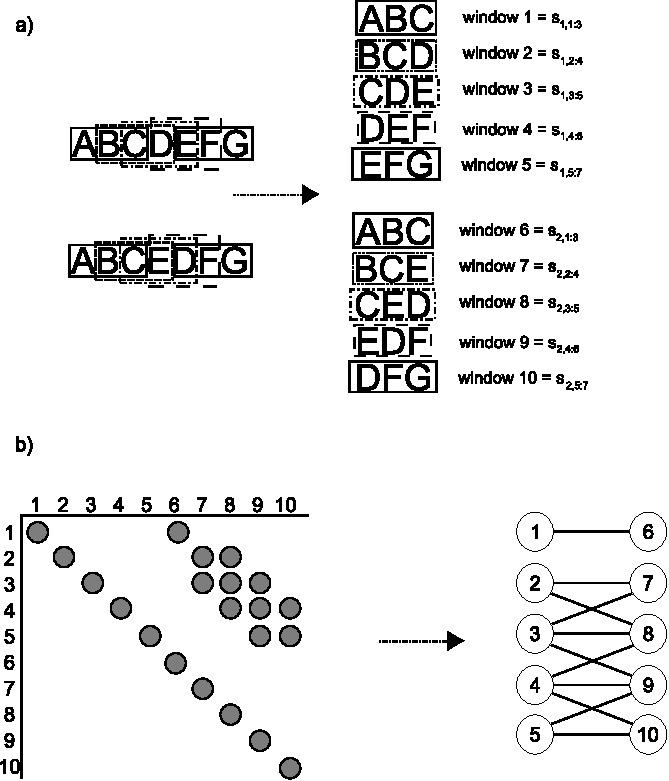
\includegraphics[width=\textwidth]{Body/Images-chap3/responseexample.pdf}
        \caption[A natural language example illustrating the
            steps that Gemoda takes]{A natural language example illustrating the
            steps that Gemoda takes.  In a), we see the three words,
        or sequences, being broken into overlapping windows of
        three letters each.  Gemoda would then compare each of these
        windows to each other using either of the similarity metrics
        described in the text.  In b), we see the resulting
        similarity matrix and how it looks when drawn as a graph.
        In the matrix, two nodes are similar by the identity metric
        if there is a dot at their intersection.  Making each window a vertex
        and connecting vertices with an edge if the windows are
        similar, we obtain the graph on the right.
        }\label{fig:response}
    \end{figure}

    Windows $3$ and $8$
    have their first letter in common, allowing them to meet the
    similarity threshold.  Windows $4$ and $9$ have their last letter
    in common, allowing them to meet the similarity threshold
    allowing the motif to extended past the letter \texttt{D}.  In the
    case of a 2--clique as in this problem, convolution reduces graphically
    to following diagonal ``streaks'' of similarity that are not on
    the main diagonal.  This streak is evident in part b of the figure.

    Giving the above--mentioned input data and parameters to Gemoda, we get
    back not only the motif that can be represented as \texttt{ABC..FG}, but
    also two other motifs that may not have been readily obvious.  The
    complete output of Gemoda is as follows:

    \begin{verbatim}
pattern 0:      len=7   sup=2   signif=1.000000e+00
    0    0       ABCDEFG
    1    0       ABCEDFG

pattern 1:      len=5   sup=2   signif=5.000000e+00
    0    1       BCDEF
    1    2       CEDFG


pattern 2:      len=5   sup=2   signif=5.000000e+00
    0    2       CDEFG
    1    1       BCEDF
\end{verbatim}

    These additional motifs are due to the low similarity threshold;
    one letter of similarity is sufficient to make three consecutive
    windows all meet the threshold.

    Now consider the same sequences with $g = 2$.
    As described
    in eariler, a motif of width $\mathscr{W}
    \ge L$ must meet the clustering and similarity
    requirements for each pair of $L$--length windows
    that is completely within the motif.  In this example,
    since the third and forth pairs of aligned windows,
    \texttt{cde \& ced} and \texttt{def \& edf}, do
    not meet the criterion of $g = 2$ for a similarity
    function based on the identity matrix, they are not
    in elementary motifs that can be convolved.  This is
    illustrated in the following diagram.

    \begin{verbatim}
       abc
       :::   --- pair 1: 3/3             ---
       abc                                 |---- maximal motif #1
        bcd                                |
        ::    --- pair 2: 2/3            ---
        bce
         cde
         :     --- pair 3: 1/3
         ced
          def
            :   --- pair 4: 1/3
          edf
           efg
            ::   --- pair 5: 2/3            ---- maximal motif #2
           dfg
    \end{verbatim}

    As shown, the first two pairs of $L=3$ length windows,
    which surpass the $g=2$ threshold, form elementary
    motifs and are convolved together.  However, because
    the third pair does not meet the criteria (and thus
    form an elementary motif) it is not convolved.
    A similar logic applies to the final two windows.
    Thus, the final, convolved, maximal motifs in this
    problem are \texttt{abc.} and \texttt{.fg}, and
    \texttt{abc..fg} is not a maximal motif motif (with $L=3,g=2$).


        \paragraph{Example 2:}
    Suppose we have a set of three words,
    \begin{eqnarray*}
        \texttt{MOTIF}\\
        \texttt{MOTOR}\\
        \texttt{POTION}
    \end{eqnarray*}
    and we would like to find the motifs that some of these words
    share in common.  Further, suppose that we are only interested
    in motifs that are at least four letters long and for which at
    least three of the four letters are ``similar'' between the windows.
    In this example, each word is a sequence, and the parameter $L$ is
    $4$.  Thus, there are $7$ possible windows that are taken
    sequentially from the three input sequences, numbered as shown in
    figure~\ref{fig:natural}.


    \begin{figure}[p!]
        \centering
        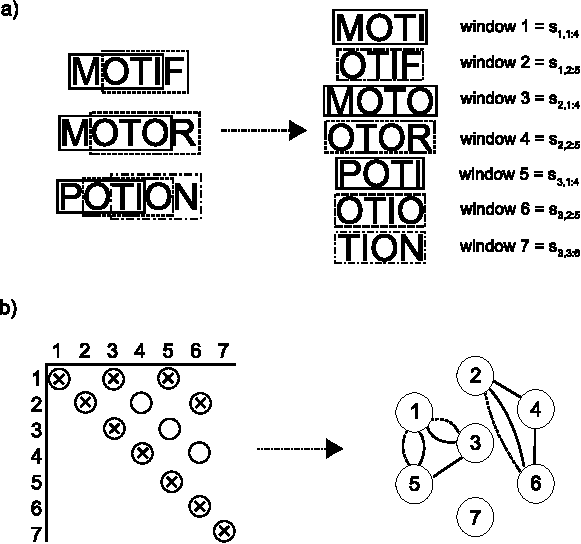
\includegraphics[width=\textwidth]{Body/Images-chap3/naturalexample.pdf}
        \caption[A second natural language example]{A second natural language example illustrating the
            steps that Gemoda takes.  In a), we see the three words,
        or sequences, being broken into overlapping windows of
        four letters each.  Gemoda would then compare each of these
        windows to each other using either of the similarity metrics
        described in the text.  In b), we see the resulting
        similarity matrix and how it looks when drawn as a graph.
        In the matrix, two nodes are similar by the identity metric
        if there is an ``X'' at their intersection, while they
        are similar by the vowel/consonant metric if there is
        an ``O'' at their intersection.  Making each window a vertex
        and connecting vertices with an edge if the windows are
        similar, we obtain the graph on the right.  Dotted lines
        indicate similarity by the identity metric, while solid
        lines indicate similarity by the vowel/consonant metric.  In
        this representation, it is clear what the results of both
        clique--finding and commutative clustering methods will be.
        }\label{fig:natural}
    \end{figure}

    If we choose a similarity function based on the identity
    matrix with a threshold of three --- that is, for two windows
    to be similar, at least three letters must be the same ---
    then we find that only the following pairs of windows are similar:
    $(1, 3)$, $(1, 5)$, and $(2, 6)$.  Importantly, we note that though
    window $1$ is similar to both windows $3$ and $5$, windows $3$ and
    $5$ are not similar to each other.

    If, on the other hand, we choose a similarity function based on
    a matrix that distinguishes only between vowels and consonants ---
    that is, any vowel is considered similar to any other vowel, and
    the same goes for any consonant --- we would see different results
    for the same threshold value.  In this case, we would find the
    following set of similarities: $(1, 3)$, $(1, 5)$, $(3, 5)$,
    $(2, 4)$, $(2, 6)$, and $(4, 6)$.

    Given these similarity matrices for the different similarity
    functions, we can now cluster the graphs.  Using the similarity
    matrix from the identity function, a clique--finding algorithm
    would find no cliques larger than size $2$; that is, the only
    cliques that exist are the pairs of similar nodes.  Since window
    $3$ (\texttt{MOTO}) is not similar to window $5$ (\texttt{POTI}),
    they cannot be in the same cluster.

    However, if we use the similarity matrix produced by the weaker
    vowel/consonant function, we will find exactly two cliques of size
    $3$: $\{1, 3, 5\}$ and $\{2, 4, 6\}$.  Though there exist pairs of nodes
    that are similar, none of them is a clique because they are not
    maximal --- that is, each individual pair of nodes that is similar
    (e.g., $(1, 3)$) can have another node added to its set ($5$) without
    violating the pairwise similarity constraint, so only the larger
    set is a clique.

    We also note that applying a connected components clustering function
    to the matrix created by the identity function would give still
    different results.  In the connected components clustering function, the
    fact that windows $3$ and $5$ are not similar would not prevent
    them from being in the same motif; the function finds all disjoint
    subgraphs and defines them as the motifs.  The motifs for such
    a case would be $\{1, 3, 5\}$ and $\{2, 6\}$, which we will call motifs
    $c_0^L$ and $c_1^L$, respectively.

    Finally, we perform the convolution step.  Using the last
    set of motifs described (with connected components clustering and
    the identity similarity function), we perform the convolution
    operation on each ordered pair of motifs; in this case, it means
    performing $c_0^L \conv c_1^L$, $c_1^L \conv c_0^L$,
    $c_1^L \conv c_1^L$, and $c_0^L \conv c_0^L$.
    For the first operation, we find the windows immediately after
    each of the windows in $c_0^L$, which is the set $\{2, 4, 6\}$.
    The intersection of this set with motif $c_1^L$ is the convolved
    motif of length $L+1$, which is $\{2, 6\}$; we can call this
    $c_0^{L+1}$.  In performing $c_1^L
    \conv c_0^L$ and $c_1^L \conv c_1^L$,
    we note that no windows exist ``after'' windows $2$
    and $6$, because their respective sequences end.  In this case,
    the first set to be intersected is null, so the intersection
    is null.  The final self--convolution operation also yields a null
    set.  We now have only one motif for the new round of convolution,
    $c_0^{L+1}$.  Performing $c_0^{L+1} \conv c_0^{L+1}$ results in
    a null set, meaning that there are no more motifs.  At this point, we
    terminate
    convolution.  It is worth noting that $c_0^L$ is returned as a
    maximal motif because window $4$ cannot be extended, but $c_1^L$ is
    not because all of its instances were convolved in one direction.

    Thus, we get different sets of motifs for different similarity and
    clustering functions.  For identity similarity and clique--finding
    clustering, the final list of motifs is
    \begin{equation*}
    \{\{\texttt{MOTIF},\texttt{POTIO}\},
      \{\texttt{MOTI},\texttt{MOTO}\}\}.
    \end{equation*}
    For identity similarity and connected components clustering, the final
    list of motifs is
    \begin{equation*}
    \{\{\texttt{MOTIF},\texttt{POTIO}\}, \{\texttt{MOTI},\texttt{MOTO},\texttt{POTI}\}\}.
    \end{equation*}
    For vowel/consonant similarity and either clustering method, the final
    list of motifs is
    \begin{equation*}
    \{\{\texttt{MOTIF},\texttt{MOTOR},\texttt{POTIO}\}\}.
    \end{equation*}



\section{Application}

    In this section, we demonstrate Gemoda's capability by presenting
    several sample applications.  Specifically, we address motif discovery
    in
    amino acid sequences, in nucleotide sequences, and in protein structures.

    As discussed previously, the clustering and convolution stages of
    the Gemoda algorithm are generic --- they are independent of the
    nature of the input data.  However, the comparison stage is
    data--specific.  In what follows, we discuss how the comparison stage
    is changed for each kind of data and outline the types of results Gemoda
    is capable of finding.

    \subsection{Motif discovery in amino acid sequences}\label{section:gemoda-aa}

    To use Gemoda to find motifs in amino acid sequences, the
    comparison stage needs to reflect the notion of
    ``similarity'' for amino acid sequences.  Specifically, we choose a
    window comparison function $\mathscr{S}$ that returns
    a sequence alignment score, such as
    the bit--score from an amino acid scoring matrix (e.g., the
    popular Blosum matrices~\citep{henikoff1992aminoacid}).

    Here, we demonstrate how Gemoda can be used
    for motif discovery in amino acid sequences
    by ``discovering'' known protein domains
    in the (ppGpp)ase family of enzymes.
    These eight enzymes catalyze the hydrolysis
    of guanosine 3',5'--bis(diphosphate) to
    guanosine 5'--diphosphate (GDP) and are
    classified by the Enzyme Commission (EC) number
    3.1.7.2~\citep{bairoch2000enzyme}.

    We used Gemoda to identify motifs in these eight
    (ppGpp)ase enzymes using the Blosum--62 scoring
    matrix as the basis of our similarity function
    $\mathscr{S}$ and the clique--based clustering
    function described previously.  Specifically, we
    sought motifs that occurred in all eight sequences,
    were at least 50 residues long, and had a pairwise
    bit--score of at least 50 bits over a window of
    50 residues.

    \begin{figure}[ptb]
        {\tiny
        \verbatiminput{Body/Images-chap3/spot.fa}
        }
        \caption[Guanosine--3',5'--bis(diphosphate)
        3'--pyrophosphohydrolase
        ((ppGpp)ase) (Penta--phosphate
        guanosine-3'--pyrophosphohydrolase)
        sequences]{Guanosine--3',5'--bis(diphosphate)
        3'--pyrophosphohydrolase
        ((ppGpp)ase) (Penta--phosphate
        guanosine-3'--pyrophosphohydrolase)
        sequences.
    These eight enzymes catalyze the hydrolysis
    of guanosine 3',5'--bis(diphosphate) to
    guanosine 5'--diphosphate (GDP) and are
    classified by the Enzyme Commission (EC) number
    3.1.7.2~\cite{bairoch2000enzyme}.
        }\label{fig:ppGppaseSeqs}
    \end{figure}

    The sequences for this example are distributed with the source
    code for the software implementation of Gemoda written by the
    authors (see Chapter~\vref{chapter:gfiles}).  Using the
    software, this example would be run as follows, assuming the protein sequences are in
    a file called ``spot.fa'':

    \bigskip
    \begin{center}
    \texttt{\$ gemoda-s -i spot.fa -l 50 -g 50 -k 8 -m BLOSUM62}
    \end{center}
    \bigskip

    With these parameters, Gemoda discovers four motifs
    in this set of eight sequences; the longest motif,
    with a length of 103 amino acids, is shown in
    Figure~\vref{fig:relaspot} as an alignment of the
    regions that correspond to instances of this motif
    (see also Figure~\ref{fig:graph}).
    A comparison with the known protein domains
    in the NCBI Conserved Domain Database (version
    2.02)~\citep{marchler2003cdd} reveals that this
    motif captures the RelA\_SpoT domain (CDD PSSM--id
    15904).


    \begin{figure}[ptb]
        \centering
        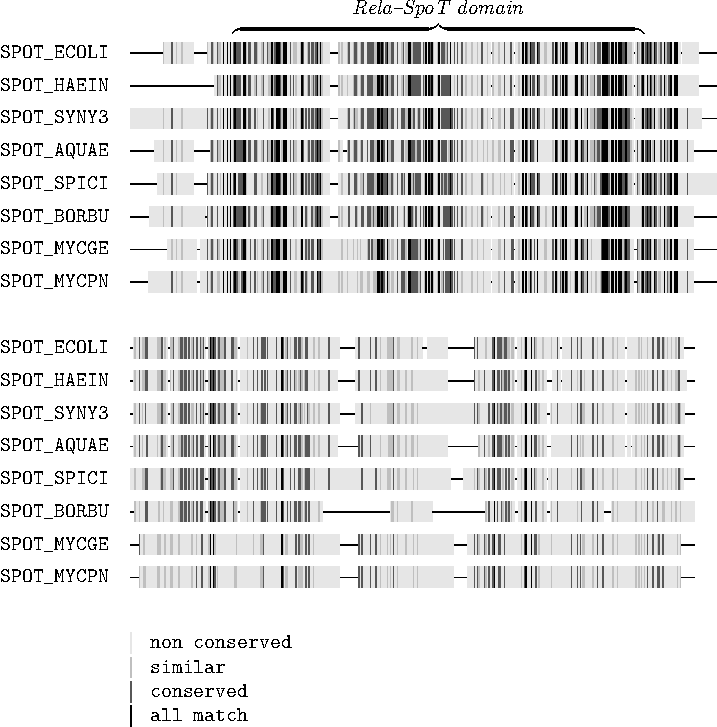
\includegraphics[width=\textwidth]{Body/Images-chap3/spot.pdf}
        \caption{The RelA\_SpoT motif detected in the 3.1.7.2 enzyme sequences.}\label{fig:relaspot}
    \end{figure}

    \begin{figure}[ptb]
        \centering
        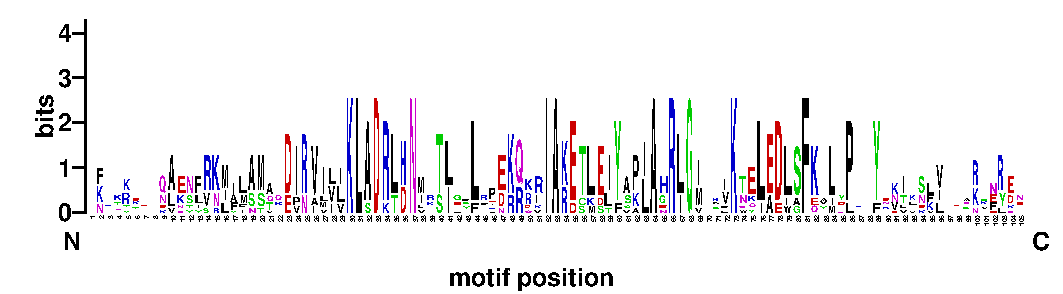
\includegraphics[width=\textwidth]{Body/Images-chap3/spot-logo.pdf}
        \caption[Logo representation of the RelA\_SpoT motif detected in the 3.1.7.2 enzyme sequences]{Logo representation of the RelA\_SpoT motif detected in the 3.1.7.2 enzyme sequences.
            In this figure, the horizontal axis represents the
            position in the motif shown in
            Figure~\vref{fig:relaspot}, in the vertical axis
            represents the information content at each position.
        }\label{fig:relaspotlogo}
    \end{figure}

    \begin{sidewaysfigure}[ptb]
        \centering
        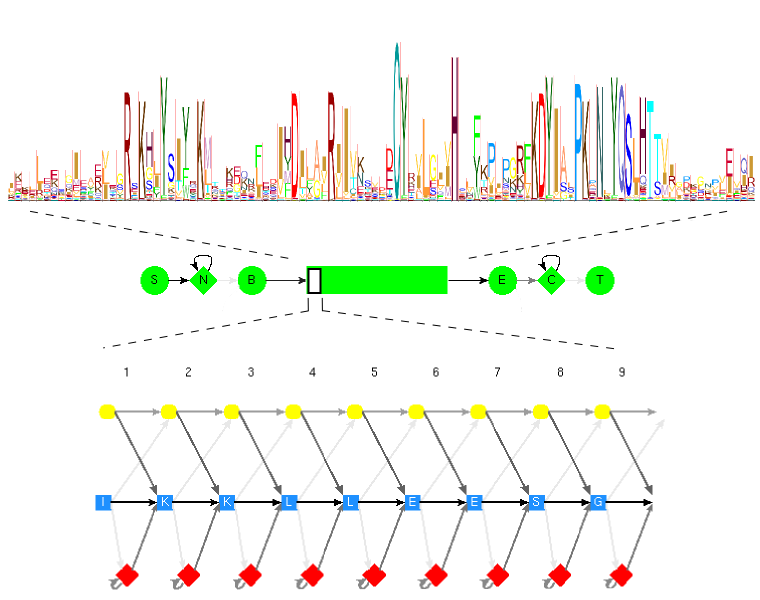
\includegraphics[height=4in]{Body/Images-chap3/hmm-graph.png}
        \caption[Logo representation of the RelA\_SpoT motif detected in the 3.1.7.2 enzyme sequences]{%
            Hidden Markov model representation of the RelA\_SpoT motif detected in the 3.1.7.2 enzyme sequences.
            In this figure, the boxes represent the different
            possible Markovian states at the first few positions in
            in the motif shown in
            Figure~\vref{fig:relaspot}~\cite{schuster2004hmm}.
        }\label{fig:relaspotlogohmmer}
    \end{sidewaysfigure}

    \begin{figure}[ptb]
        \centering
        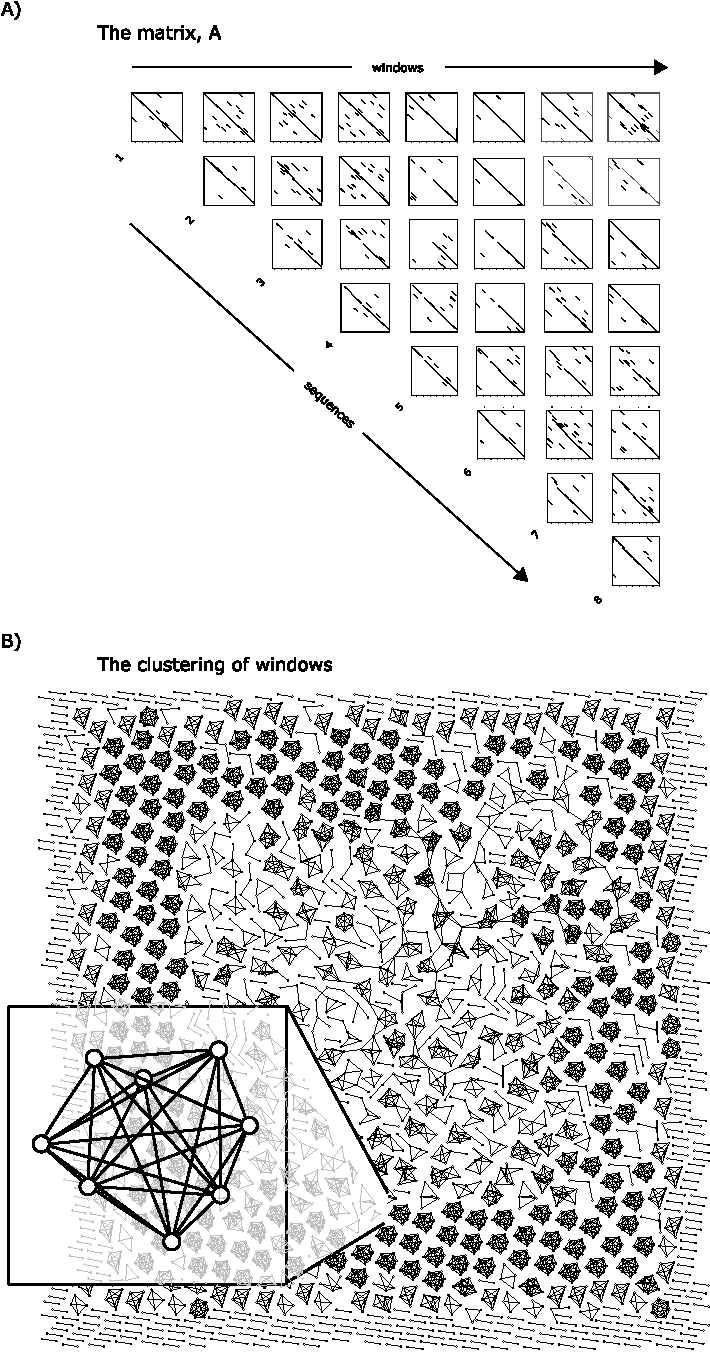
\includegraphics[height=5in]{Body/Images-chap3/gemoda_fig2.pdf}
        \caption[The similarity graph for the Gemoda 3.1.7.2 enzyme example]{The similarity graph for the 3.1.7.2 enzyme example.
            (A) is the similarity
            matrix $A$, which contains one row and column
            for each window of 50 residues in the
            set of input sequences.  Entries in the
            matrix have been thresholded such that
            pairs of windows that can be aligned
            with a bit--score greater than 20 are
            given a black dot and all others
            are white, producing the familiar
            dot--plot appearance of the matrix.
            (B) is a graph representation
            of $A$.  Each vertex represents a window,
            and two vertices
            are connected with an edge if
            they have a black dot in the top image.
            The breakout shows a clique of size
            eight, which represents a set of
            windows that participate in the motif
            shown in Figure~\vref{fig:relaspot}.
            In general, as the bit--score threshold
            is lowered, the number of edges
            in the graph increases, making the
            clustering stage more computationally
            intensive.  When using clique--based
            clustering with too small of a threshold,
            computational expense may make the problem
            infeasible.
            At these thresholds the
            ``signal'' cannot be distinguished
            from the ``noise.''  However, with
            the parameters used in this example,
            the clustering phase is quite easy,
            which is intuitive given the number
            of disjoint subgraphs shown in the
            bottom image.
            }\label{fig:graph}
    \end{figure}


    The remaining three motifs are not present in
    the CDD database.  However, further inspection
    using the tools available from the PFAM
    database~\citep{bateman2004pfam} revealed that
    they composed the left, middle, and right regions
    of the HD domain~\citep{aravind1998hd}.
    In the SpoT enzymes, this domain has a number
    of insertions and deletions that give rise to
    gaps such that Gemoda identified and reported
    individually the left, middle, and right regions
    of conservation of the HD domain.

    In this example, the Blosum--62 matrix was chosen
    as the similarity metric because it is optimized
    for detecting distant homologs.  The Gemoda
    input parameters $L=50$ and $g=50$ were
    chosen to enforce a one--bit--per--base score,
    which should rise above random ``noise'' since,
    by design, the expected bit--score for two aligned
    amino acids is negative for the Blosum set
    of scoring matrices.

    In order to test the sensitivity of these results
    to noise, we conducted an experiment to determine
    the degree to which these (ppGpp)ase motifs
    could be found if obscured by noise caused by
    adding random spurious sequences to the 8 enzyme
    sequences.  We found that, with the Gemoda input
    parameters described above and using random
    sequences selected from Swiss--Prot (Release
    45.0)~\citep{bairoch2000swiss-prot}, the target
    motifs could be detected in an 8--fold majority
    of spurious sequences.





    \subsection{Motif discovery in protein structures}

    The detection of 3--dimensional motifs in sets
    of protein structures is another
    problem type that Gemoda can address.
    Often, homologs that are related through a
    distant lineage show little to no
    sequence similarity, particularly at the nucleotide
    level~\citep{eidhammer2000structure}.  However,
    these homologs frequently show conserved tertiary
    structures~\citep{dietmass2001indentification},
    making motif discovery in protein structures often
    revealing in situations where there appears to
    be no similarity at a sequence level.

    There are a number of well--developed tools for
    the pair--wise comparison of protein structures
    or the comparison of a single protein structure to
    precomputed structural motifs; these have been reviewed
    elsewhere~\citep{eidhammer2000structure}.
    Some of the more popular tools
    include SSAP~\citep{orengo1996ssap},
    VAST~\citep{madej1995threading},
    Dali~\citep{holm1993protein},
    and Mammoth~\citep{ortiz2002mammoth}.
    The Gemoda algorithm, when used for structural
    motif discovery, is most similar to the
    Sarf algorithm~\citep{alexandrov1996sarfing,alexandrov1996analysis}
    and, to a lesser degree, algorithms
    by~\citep{hunter2003protein}
    and~\citep{jonassen2002structure}.
    Conceptually, Gemoda could be thought of as a hybrid
    of the Sarf and Teiresias algorithms, combining
    3--D elementary motif discovery with convolution.
    To the best of our knowledge, Gemoda is the only tool that can
    compare an arbitrary number of protein structures
    simultaneously and produce an exhaustive set of
    maximal motifs.

    To discover motifs in protein structures,
    Gemoda compares $L$--residue windows of the
    proteins' alpha--carbon trace using the
    minimized RMSD similarity metric (one of
    many possible metrics for comparing protein
    sub--structures~\citep{kolodny2005comprehensive}).
    Here we use ``minimized'' to indicate
    that the protein structures are optimally
    super--imposed via rigid--body rotation and
    translation~\citep{horn1987closed,arun1987least};
    occasionally this term is implicit.  Using the
    clique--finding clustering algorithm, Gemoda finds
    motifs that are sets of alpha--carbon traces (in
    a set of protein structures) that can be super--imposed
    with an RMSD less than $g$ $\AA$ over each window
    of $L$ residues on a
    pair--wise basis.  Similar to the amino acid and
    nucleotide applications of Gemoda, these structural
    motifs are maximal in both length and support.

    Here, we demonstrate how the Gemoda algorithm
    can be used for structural motif discovery by
    ``discovering'' the structural homology between the
    human galactose-1-phosphate uridylyltransferase
    (PDB id 1HXQ)~\citep{wedekind1996structure}
    and fragile histidine triad proteins (PDB id
    3FIT)~\citep{lima1997mad}, originally reported
    elsewhere~\citep{holm1997enzyme}.  Using Gemoda,
    we looked for motifs of at least 30 residues,
    occurring in at least three chains, that had a
    pairwise RMSD of 1.5 $\AA$ or less (based on
    superposition of the alpha--carbon backbone)
    over each window of 30 residues.

    This search returns 4 motifs, the longest of
    which is 66 residues (see Figure~\vref{fig:holm}).
    This motif has one embedding in the 3FIT protein
    and two, in different chains, in the 1HXQ protein.
    As shown in the figure, the motif is an alpha helix
    followed by a beta sheet.

    \begin{figure}[ptb]
        \centering
        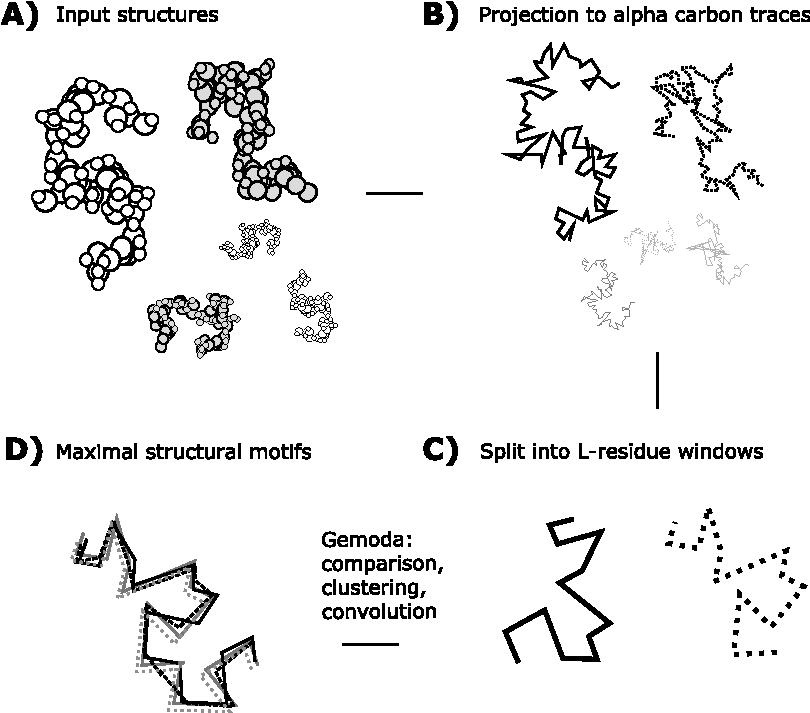
\includegraphics[width=0.90\textwidth]{Body/Images-chap3/rmsd.pdf}
        \caption[Alpha carbon trace projection used  by Gemoda]{Alpha carbon trace projection used  by Gemoda}
        \label{fig:trace}
    \end{figure}

    \begin{figure}[ptb]
        \centering
        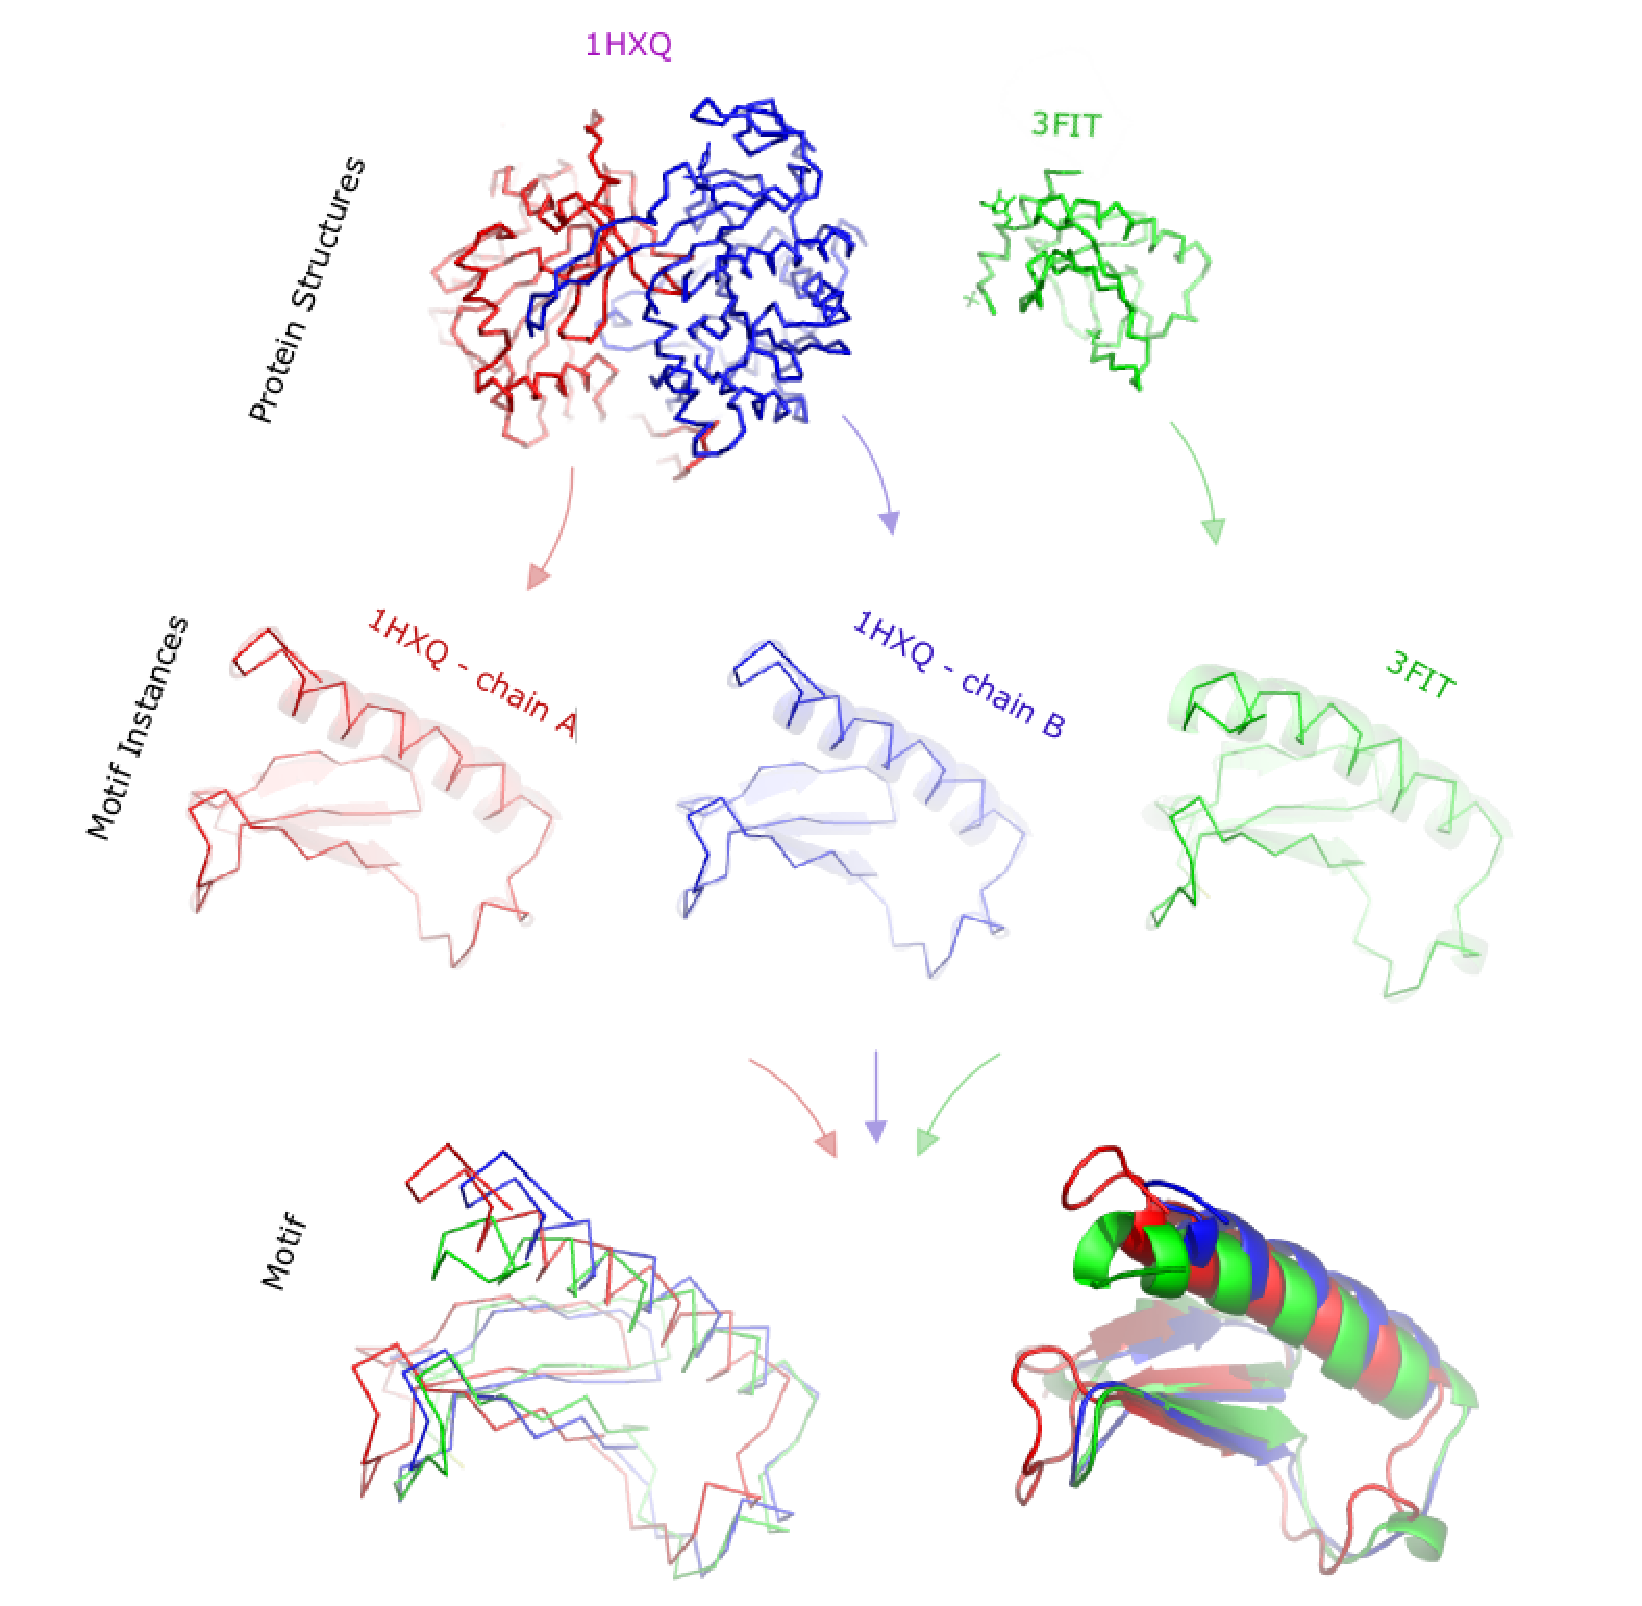
\includegraphics[width=0.90\textwidth]{Body/Images-chap3/gemoda_fig4.pdf}
        \caption[A motif showing structural conservation between
        the human galactose-1-phosphate uridylyltransferase and
        fragile histidine triad proteins originally reported
        by~\citet{holm1997enzyme}]{A motif showing structural conservation between
        the human galactose-1-phosphate uridylyltransferase and
        fragile histidine triad proteins originally reported
        by~\citet{holm1997enzyme}.
        The motif, as shown here, was ``discovered''
        using the Gemoda algorithm along with three other, smaller,
        structural motifs that are highly conserved between the
        two proteins.  Notably, the proteins show little sequence
        similarity over the region displayed in the structural
        motif above.  Graphics created using PyMol (DeLano Scientific,
        San Carlos, CA, USA).  See also Figure~\vref{fig:holmViewer}.}\label{fig:holm}
    \end{figure}

    \begin{figure}[ptb]
        \centering
        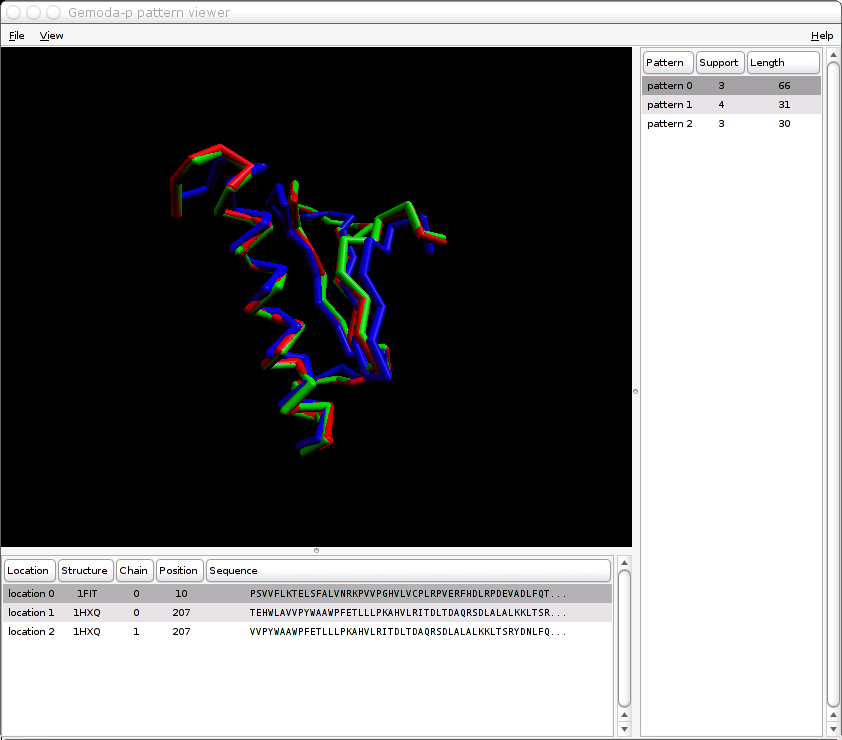
\includegraphics[width=0.90\textwidth]{Body/Images-chap3/galt-hit.png}
        \caption[Structural motif in Gemoda's 3--D structure viewer]{The
            human galactose-1-phosphate uridylyltransferase and
        fragile histidine triad structural motif (see Figure~\vref{fig:holm}) in Gemoda's 3--D structure viewer,
        which was written by the authors for viewing output from gemoda--p.
        }\label{fig:holmViewer}
    \end{figure}


    \subsection{Motif discovery in nucleotide sequences and the (\textit{l,d})--motif problem}



    \subsubsection{Introduction}
        Four years ago, Pevzner and Sze~\cite{pevzner2000combinatorial} noted
    that despite significant advances in pattern discovery,
    there were still gaping holes in our ability to identify and
    enumerate frequent patterns in biological sequences.
    Experimental noise and error were not the only significant issues,
    as the community was still incapable of solving certain
    problems with purely synthetic data and no worry of experimental or
    gross error.  One such problem, defined below, was the (\textit{l,d})--motif
    challenge problem; it exposed the fact that certain motifs, despite
    having a strong consensus and being rather unlikely to occur at random in
    independent and identically distributed (i.i.d.) sequences,
    are extremely hard for most motif discovery algorithms
    to locate.  The reason that these motifs are hard to locate is that even
    though they may deviate very little from a consensus sequence, their pairwise
    deviation tends to be rather large.  Other false pairwise similarities
    are thus extremely likely to occur at random elsewhere in the dataset, and
    this random noise obscures the true motif's signal.  Pevzner
    and Sze~\cite{pevzner2000combinatorial} presented two algorithms that looked towards solving this
    problem; Buhler and Tompa~\cite{buhler2001finding} followed suit by presenting a more effective
    algorithm.  However, the problem is still not completely solved per se;
    difficulties exist in obtaining the correctly refined motifs and instances even for this
    simplified model of biology.  In addition, though existing algorithms
    move towards solving this simplified problem,
    they are not nearly as helpful in addressing the biological realities
    that computational biologists face.

        The original (\textit{l,d})--motif problem \cite{pevzner2000combinatorial}~
    can be paraphrased as follows:
    \begin{quotation}
    Within a set of random DNA sequences with i.i.d\ nucleotides,
    a parent motif of length $l$ is embedded in each sequence in a
    random location.  Each time the motif is embedded, it is
    mutated in $d$ locations.  The (\textit{l,d})--motif problem is to recover
    the locations of the embeddings, knowing only the parameters $l$
    and $d$ and that each sequence contains exactly one
    instance of the motif.
    \end{quotation}

    At first, this seems to be a reasonable simplification of the phenomenon of
    binding sites and other functional sites in DNA.  It is not uncommon to have
    some ancestral sequence from which each motif occurrence is some short
    evolutionary distance away.  This model accurately captures the
    difference between instance--instance similarity and instance--ancestor
    similarity.  That is, even though a motif instance may be a very short
    distance from its ancestor (say, four mutations out of fifteen bases), any
    two instances of the motif may be significantly different from each other
    (eight mutations out of fifteen bases).  This low degree of instance--instance
    similarity can occur rather frequently in random i.i.d. nucleotide
    sequences, thus obscuring the true evolutionary relationship of the
    motif instances (the signal) with purely random relationships of background
    nucleotides (the noise) \cite{buhler2001finding,buhler2002finding}.

    As discussed by Buhler and Tompa~\cite{buhler2001finding}, local search methods (such as the
    common ones mentioned before) using typical initialization strategies
    encounter an insurmountable amount of noise when searching for some sparse motifs
    described by the (\textit{l,d})--motif problem.  We would ideally like
    to be able to recover such motifs, since they are expected to occur by chance
    in every sequence with rather low probability (approximately
    $10^{-7}$)~\cite{buhler2001finding,buhler2002finding}.

    In a more realistic scenario, a researcher may not know the size $l$
    of the motif \textit{a priori}.  Instead, it is more likely that she
    would know the evolutionary distance between motif instances, i.e.\
    the rate of mutation $d/l$.  It is also unrealistic to mutate
    the embedded motif \textit{exactly} $d$ times; rather, the researcher
    is more likely to be interested in motifs that are $d$ or fewer mutations
    away from each other.  That is, in a real--world senario, we would
    more likely have a reasonable estimate of the upper limit $d/l$ of the mutation distance
     between embedded motifs.
    There may also be multiple, different motifs in the dataset.  Finally,
    as experimental data are
    commonly rife with noise, it is likely that some of the sequences
    may be false--positive candidates for the motif; that is, some sequences may
    contain no motifs at all.

    With these issues in mind, we define an extended (\textit{l,d})--motif problem
    as follows:
    \begin{quotation}
    Within a set of random DNA sequences with i.i.d.\
    nucleotides, a parent motif of length $\geq L$
    is embedded zero or more times in each sequence in
    a random location, such that the motif has been
    embedded a total of $k$ times in the data set.
    Also, each time the motif is embedded it is mutated
    such that there are no more than $d$ mutations over
    any window of $l$ nucleotides (that is, the rate of mutation is $d/l$).
    This process is
    repeated for any number of parent motifs, each with
    the same $l$ and $d$, but possibly different $L$.
    The extended (\textit{l,d})--motif problem is to recover the
    locations of the embeddings for every parent motif
    without any \textit{a priori} knowledge of where
    they might be, but only knowing the parameters $l$ and $d$.
    \end{quotation}
    We will refer to this formulation as the ``extended'' (\textit{l,d})--motif
    problem and the previous formulation as the ``restricted''
    (\textit{l,d})--motif problem.  In what follows, we detail an algorithm
    for solving both the extended and restricted (\textit{l,d})--motif problems.

    We say that a motif, $p$, is just a data structure with two features:
    a width, $\mathscr{W}(p)$, and a list of locations in the data
    where the motif has been embedded, $\mathscr{L}(p)$.  A motif has
    the property that the locations in $\mathscr{L}(p)$ are all within a
    Hamming distance of $2d$ from each other over every window of size $l$.

        We will call the Hamming distance function
    $\mathscr{H}$, where $\mathscr{H}$
    takes two windows of size $l$ from our sequence set,
    and returns a real--valued number equal to the
    number of characters that differ between the two windows.


    \subsubsection{Solving the restricted (\textit{l,d})--motif problem}
        The input set for the (\textit{l,d})--motif problem is any arbitrary set of $n$
    sequences, each with length $W_i$ nucleotides.  Most bioinformatics
    literature treatments use $W_i=600$ and $n=20$.  Different versions of
    this problem have been discussed at length; the most commonly discussed
    is the (15,4) problem, while the (14,4) and other associated, more
    difficult problems are also addressed in the literature.

    It has been shown before that the most commonly used motif discovery
    algorithms, including CONSENSUS~\cite{hertz1999identifying}, Gibbs
    sampling~\cite{lawrence1993detecting}, and
    MEME~\cite{bailey1994fitting}, are unable to
    solve the restricted (15,4) problem.  Algorithms that are capable of solving the
    restricted (15,4) problem have been presented in the literature.  While some of
    these, including Winnower and SP-STAR~\cite{pevzner2000combinatorial},
    are unable to solve the more
    complicated (14,4) problems, others are able to address this and other,
    more difficult, problems with some degree of accuracy.  These latter
    algorithms usually leave the deterministic realm, though, and rely on
    probabilistic methods to find the planted motifs.

    On the other hand, our algorithm allows for exhaustive, deterministic solution of these
    problems.  The (\textit{l,d})--motif problem solved by the
    above--mentioned tools is a degenerate case of the extended problem
    that our algorithm was designed to solve.  Thus, our algorithm is not optimally tuned
    for solving the
    restricted (\textit{l,d})--motif problem in the least amount of time.
    Nonetheless, solving a range of the restricted (\textit{l,d})--motif problems
    is still a valuable check on the utility
    of our tool to make sure it can solve at least some of them in a
    reasonable amount of time.  In addition, our exhaustive
    search allows for one to see how many other false signals are in
    the data.  This can facilitate the assessment of statistical
    significance of results, certainly an
    important step in analyzing any proposed signal.

    Our algorithm requires three user input parameters: $l$, $g$, and $k$.  $l$ is the
    minimum motif size and the size of the sliding window used for judging
    similarity between two sequences.  $g$ is the similarity threshold
    for any two windows to be deemed instances of the same motif; in this case,
     if two windows
    of length 10 are a Hamming distance of 2 away from each other, $g$ would need
    to be 8 or less for the windows to be in the same motif.  Finally,
    $k$ is the support, or minimum number of motif occurrences required
    to report the motif to the user.

    It is obvious that any two motifs of length $l$ each being mutated $d$
    times from an ancestral sequence can differ at most at $2d$ locations.
    Thus, at least ($l-2d$) locations must be preserved in the motif.
    This observation lays the foundation for discovery of the hidden motifs.
    Our algorithm is run with parameters $l=15$, $g=7$, and $k=20$
    for the (15,4) problem.  The discovery of the motif is then a
    straightforward combinatorial problem with deterministic
    discovery of the solution.

    It is important to note, however,
    that our method will solve and return a superset of the restricted
    (\textit{l,d})--motif problem.  That is, any group of $d$--mutants from a
    common ancestor can be described as having ($l-2d$) identical bases, but
    not all groups of sequences with ($l-2d$) identical bases can be used to
    synthesize an ancestor from which all group members deviate $\leq d$ bases.
    When there are a large number of ``signal'' motif members, there
    is usually sufficient overall deviation to prevent a $\geq d$--mutant from
    joining a motif group.  However, at smaller support $k$, it is more likely
    to find motif instances that violate the $d$--mutant constraint.  It is not
    desirable to immediately remove motifs with such members from the output, as they
    do still meet the constraints imposed by our parameter values; rather, we
    can use a simple post-processing method to note which motifs have readily
    obvious ancestors and thus are the most likely candidate signals.

    A few interesting observations can be made regarding the complexity of
    the algorithm and the quality of its solutions.  First
    of all, the time to solution is not affected directly by the
    length of the motif to be discovered as in many other exhaustive methods.
    Rather, it is the sparseness or subtlety of the
    motif (or more accurately, the probability of the pairwise motif similarity occurring
    randomly) that has the most profound impact on the complexity of the
    algorithm.  The most computationally expensive step is the clique-finding
    function, which
    increases in computation time with the number of edges (np--complexity at worst,
    though on average much better).
    For varying $l$ and $d$, as two $l$-mers sampled randomly from
    the background are more likely to meet the threshold of similarity defined by
    $l$ and $d$, there will be more false edges (similarities) in the graph,
    and thus the clustering algorithm will take longer.  Motifs of widely different
    length may be (approximately) equally likely in the background
    distribution if $d$ is set to a certain value for each.  In this case, it
    would take almost exactly the same amount of time to find both motifs in
    the same input set.  Of course, the size of the data set also has a
    significant impact on computation time, as for
    any algorithm; a larger input set
    causes more false occurrences of a potential motif,
    and the resulting distance matrix needs
    more time to be explored by our clique-finding algorithm.

    Also, our method does not preclude discovery of more than one instance of a
    motif in any given sequence.  Much
    like the re--framing of the (\textit{l,d})--motif problem presented above,
    this is more
    reflective of what one expects may happen in a real biological system:
    motifs of biological significance may occur more than once in a
    biosequence, and it behooves us to be able to discover all occurrences.
    In fact, in the original dataset for the (15,4)--motif problem used by
    Pevzner and Sze~\cite{pevzner2000combinatorial}, there is actually an additional
    instance of the original
    motif that occurred completely by chance; this instance was discovered in
    our solution of the problem.    With
    Gemoda, we can easily identify this instance without any
    additional work or manipulation.
    The sequence logo for the planted motif from
    Pevzner and Sze's initial dataset is shown in
    Figure \vref{fig:MCP}; the consensus sequence
    is \texttt{GGCTTTGTAGCTAAC}.  The ``accidental''
    instance of the embedded motif that can be identified
    using
    Gemoda is \texttt{GGATTGATAGCTAAG}.

    Finally, it is important to note the absolute accuracy of our results.
    In previous papers presenting algorithms to solve
    the (\textit{l,d})--motif problem, a metric called the performance coefficient is used
    to gauge the accuracy of the algorithms.  This is defined as
    $ \frac{K \cap P}{K \cup P}$, where K is the set of $l*s$ nucleotides
    representing the $s$ motif instances each of length $l$ and P is
    the set of $l*s$
    nucleotides representing the $s$ proposed motif instances of length $l$.
    Coefficients above .75 are usually deemed acceptable for these algorithms.
    Improved algorithms return results with coefficients of about 0.9 or 0.95.
    Examples of the performance of other algorithms are presented in
    Table~\ref{table:performance}.   Clearly, our algorithm returns all coefficients of 1; that
    is, it will return the exact location of all motif occurrences.  This is
    a notable improvement over other algorithms that may return approximate
    motif locations that then need to be verified and slightly adjusted or
    optimized by hand.  In fact, in any given run of PROJECTION (the most accurate
    of the algorithms in Table~\ref{table:performance}), one will usually find
    that one or two (or even more) of the returned motif instances are
    not just imperfectly located, but are false positives.

\begin{sidewaystable}[h]
\caption[Performance on a range of (\textit{l,d})--motif problems with synthetic data]{Performance on a range of (\textit{l,d})--motif problems with synthetic data.
Data from other algorithms are from
Buhler and Tompa~\cite{buhler2002finding}.  GibbsDNA, WINNOWER, and SP-STAR are averaged over
eight random instances, while PROJECTION is averaged over 100 random instances.  Computation
times for our proposed algorithm are averaged over three random instances.}
\label{table:performance}
\begin{center}
\begin{tabular}{cc|cccc|cc} \hline
$l$ & $d$   & GibbsDNA & WINNOWER & SP-STAR & PROJECTION & Proposed algorithm & Time\\ \hline
10  & 2 & 0.20  & 0.78  & 0.56  & 0.80  & 1.00  & 8 min\\
11  & 2 & 0.68  & 0.90  & 0.84  & 0.94  & 1.00  & $\lt1$ min\\
12  & 3 & 0.03  & 0.75  & 0.33  & 0.77  & 1.00  & 10.5 h\\
13  & 3 & 0.60  & 0.92  & 0.92  & 0.94  & 1.00  & 10 min\\
14  & 4 & 0.02  & 0.02  & 0.20  & 0.71  & 1.00  & $\gt3$ months\\
15  & 4 & 0.19  & 0.92  & 0.73  & 0.93  & 1.00  & 6 h\\
17  & 5 & 0.28  & 0.03  & 0.69  & 0.93  & 1.00  & 3 weeks\\ \hline
\end{tabular}
\end{center}
\end{sidewaystable}

    The computation time of our tool becomes unacceptable
    as the motifs become degraded beyond the (15,4) problem.  This is to be
    expected for a deterministic algorithm as the probability of the signal
    reaches a level that causes many pairwise similarities to occur by chance.
    Since our strategy is generalized and exhaustive,
    we expect the computation times to be suboptimal.  Beyond this table,
    one would benefit from other probabilistic or heuristic algorithms in order
    to solve the more difficult (\textit{l,d})--motif problems in an acceptable
    period of time.  Fortunately, it seems to not be a too frequent occurrence to
    search for a (18,6)--motif in each of 20 biological sequences, so our algorithm
    should be of significant utility for common applications.

\subsubsection{Solving the extended problem}
    Of course, in a real biological problem, one does not have nearly the
    same certainty in the contents of each biosequence as is allowed by the
    (\textit{l,d})--motif problem.  This becomes evident upon analyzing the situations
    that the (\textit{l,d})--motif problem is meant to analyze, the most salient of which
    being the discovery of transcription factor binding sites.  In order to
    come up with the candidate coregulated sequences, the results of
    laboratory experiments are analyzed to find which genes are sufficiently
    coexpressed.  However, much of this data is prone to noise.
    Some genes may not be coexpressed, though they may seem to be
    due to some experimental aberration.  Of those that are actually
    coexpressed, they may or may not be coregulated by the same transcription
    factor; it is a distinct possibility (and quite frequently a reality)
    that genes appearing to be coexpressed are not bound by any common
    factor.  The same analysis follows for other situations for which the
    (\textit{l,d})--motif problem is an otherwise reasonable approximation: experimental
    noise prevents certainty that all input sequences are truly.

    Other methods meant to be robust enough to solve
    the restricted (\textit{l,d})--motif problem will lose significant
    advantage in this more realistic, extended set of circumstances.
    Our algorithm was designed specifically to deal with the issues addressed by the
    extended challenge problem.  It discovers, in a provably exhaustive and
    deterministic fashion, all motifs described in the
    extended problem definition.  Other algorithms discussed
    previously in this paper are just not constructed to deal with such
    uncertainty in motif characteristics; as such, there is little way to
    accurately compare the performance of ours and other algorithms on the
    fully extended problem.
    Thus, it seems intuitive to simplify the extended problem to
    something more complicated than the restricted (\textit{l,d})--motif problem,
    but for which there is still a useful metric for comparison between ours and
    other algorithms.
    What follows are two cases (discussed qualitatively)
    which demonstrate
    the specific benefits of our tool for pattern discovery on (15,4) problems
    beyond the restricted version.

    \paragraph{Case 1: An underestimated number of motif instances.}
    One source of difficulty in the extended problem may be
    the uncertainty as to the exact number of motif instances.  For this
    case, we still restrict ourselves to windows of size $l$ with $d$ mutations
    from a consensus sequence.  However, we allow for uncertainty in the number
    of motif instances.
    For
    this case study, we instruct algorithms to find motifs with instances in at
    least 15 sequences when in fact there is an instance in every sequence.  If
    an algorithm such as WINNOWER were to search for cliques across 15 sequences
    when in fact all 20 sequences had a motif instance, it would have a
    final graph with much more than the single signal that it usually hopes to
    obtain.  PROJECTION's attempts to find 15
    instances when 20 actually occur are similarly problem-ridden, returning
    different candidate motifs on different runs.  These results would sometimes have
    significant overlap with initial planted motif, though at other times would
    have very little overlap.  Most disturbingly, all of these proposed motifs
    would have approximately the same score, thus making it difficult to discern
    a truly useful motif from one constructed from background noise.  Our algorithm,
    on the other hand, returned the initially planted motif along with other smaller
    patterns that still met the criteria for classification as a motif.

    \paragraph{Case 2: Zero-or-one motif instances.}
    In this next case, we analyze the impact of there being zero or one motif
    instances in each sequence.  To implement this simplification, we instruct
    each algorithm to find the exactly 15 motif instances that are implanted across 20
    sequences.  This makes the problem astonishingly similar to the
    (\textit{l,d})--motif problem, with the exception that not every sequence
    contains a motif instance.  This problem setup is thus significantly more
    realistic, as one does not expect every sequence to have a motif occurrence
    in every pattern discovery problem.  Of course, this is still a simplification
    of reality, as one would not expect to know the exact number of motif
    instances.  However, not even this
    gross simplification can salvage the efficacy of existing algorithms for
    the discovery of such subtle motifs.  A
    study using PROJECTION found results that rarely approached acceptable levels and
    more frequently approached performance coefficients
    expected from purely random guessing.  Again, though, our algorithm solved
    the problem with only a small increase in computation time over solving the
    original (\textit{l,d})--motif problem.

    \subsubsection{Identifying natural cis--regulatory elements}
    For some regulons in \textit{E. coli} with mild
    to strong consensus sequences, Gemoda returns
    results that are similar to or improve upon the
    results from commonly--used motif discovery tools.
    For instance, using the set of upstream regions
    ($400$ base pairs upstream and $50$ base pairs
    downstream of the translation start site) for
    the $9$ operons believed to be regulated by
    LexA~\citep{salgado2004regulondb}, Gemoda's
    top--scoring motif was used to generate the
    sequence logo found in Figure \vref{fig:MCP}.
    This motif closely matches the literature PWM
    for the LexA binding site and represents 80\%
    of the literature--found binding sites with no
    false positives.  Of course, the difficulty of DNA motif
    discovery problems varies greatly, and this is only one
    straightforward example of such problems.

    \begin{figure}[ptb]
        \centering
        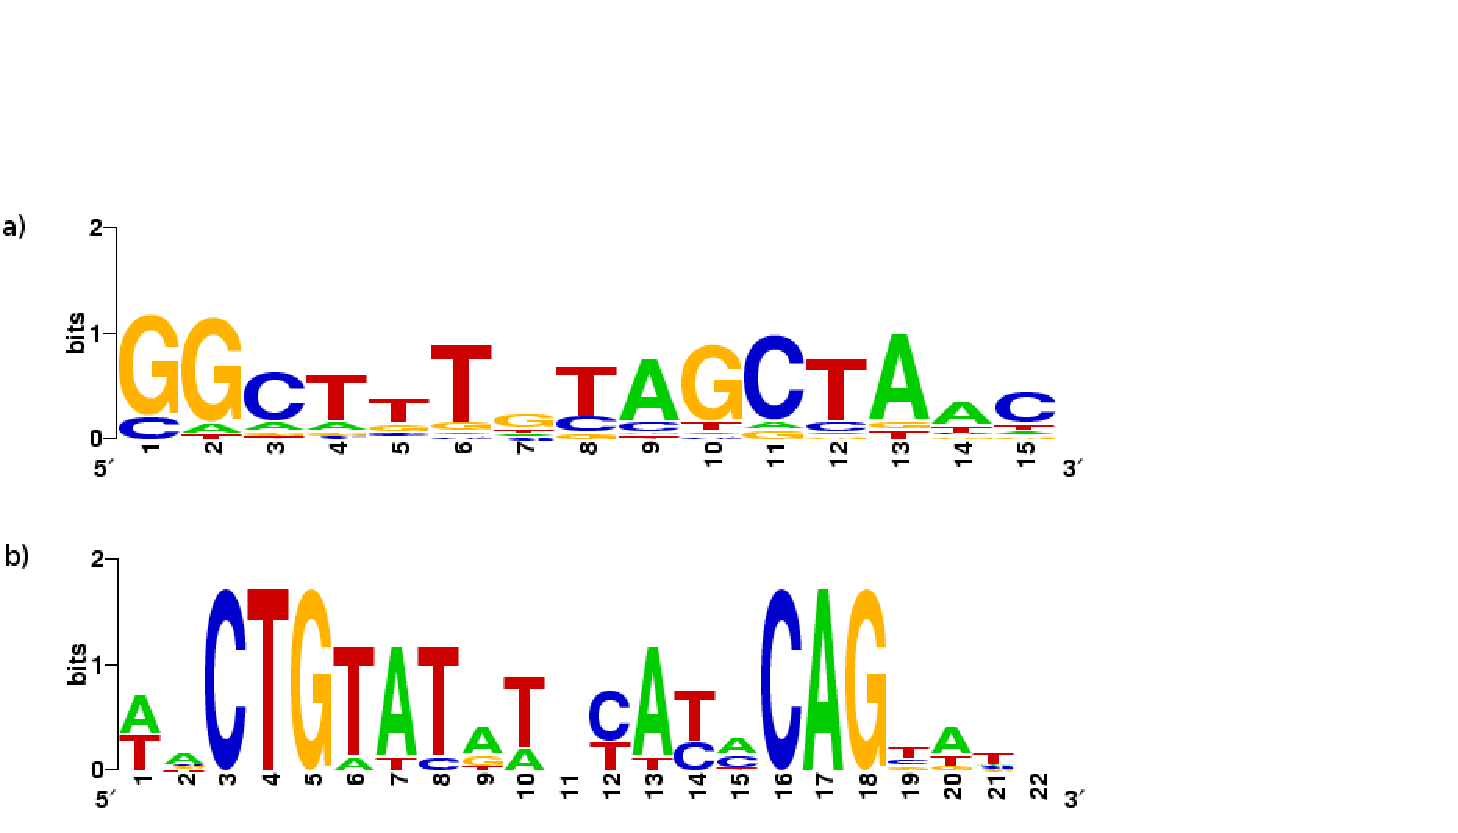
\includegraphics[width=0.40\textwidth]{Body/Images-chap3/gemoda_fig3.pdf}
        \caption{The sequence logo for a) the motif implanted in each
            sequence for the (\textit{l,d})--motif problem and b) the
        LexA binding site motif generated from the highest--scoring
        motif returned by Gemoda.}\label{fig:MCP}
    \end{figure}

    The parameters used for this search were $L = 20$, $g = 10$, and
    $k = 6$ with the identity matrix scoring scheme
    and clique--based clustering described above.
    The length was selected based on the knowledge
    that the DNA--binding domain of LexA is a
    helix--turn--helix variant, and so it was likely
    to be a relatively long motif.  The similarity
    threshold was chosen as one--half of $L$, which
    we know from the (\textit{l,d})--motif problem
    ought to be approximately sufficient to prevent
    the graph from being too dense (and thus expensive
    to cluster).  The support threshold was chosen to
    be about two--thirds the total number of sequences,
    allowing for some noise in the data.  Of course,
    the judicious selection of parameters is an
    outstanding problem in binding site discovery.
    It is worth noting that most of these selections
    were simple or intuitive and that there was some tolerance
    in the results for slight perturbations in parameters.

\subsubsection{Conclusions}
    The benefit of our proposed algorithm is then obvious:
    deterministic and provably complete
    output even in the face of uncertainty in motif characteristics.  The motifs
    could have been longer than 15 bases, could have had fewer mutations, or
    could have occurred in a variable number of sequences, and our tool would
    have found them.  Its only obvious negative aspect is its
    computational expense.  The restricted (15,4) problem took 6 hours, while the
    extended problem took 13 hours.  Compared to the runtimes of algorithms
    like PROJECTION, which can be as low as five minutes for the restricted
    problem, these runtimes may seem extremely large.  In practice, however, this
    computation time is far from unacceptable; one would not expect to often
    encounter the need to run motif discovery many times sequentially,
    particularly if the results being returned to the user are
    deterministically correct.

    Perhaps even more importantly, we have reframed the challenge problem
    statement in a way that is more biologically meaningful; hopefully this
    new challenge will inspire other methods that outperform ours in some way.
    While a deterministic and exhaustive method is always welcome,
    for some problems it seems that a heuristic approach may provide a
    good balance between time and accuracy; we look forward to seeing
    new tools that address our amended problem with sufficient accuracy.




\section{Discussion}

Gemoda makes four contributions.  First, the
algorithm is generic in that it is equally applicable to
any variety of sequential data.  Second, Gemoda allows
arbitrary similarity metrics.  In the examples shown here,
we chose relatively simple metrics (scoring matrices and
RMSD--base metrics); however, similarity metrics can
be easily changed or added. For example, in the case of amino acid
sequences, one can easily define hybrid metrics
incorporating primary, secondary, and tertiary structure
features.  In the case of nucleotide sequences,
the metric may be changed to incorporate methylation information.
The third contribution is that Gemoda
returns motifs that are not tied
to any particular motif representation.  In
the case of amino acid sequence motifs, it is easy to model
Gemoda's motifs using regular expressions, hidden Markov
models, or position--specific scoring matrices.  Finally,
when used with the clique--finding clustering algorithm,
Gemoda returns an exhaustive set of maximal motifs.
To the best of our knowledge, Gemoda is the only motif discovery
algorithm incorporating the above features.

As mentioned in the introduction, Gemoda integrates the
best characteristics from a number of previously published
motif and association discovery algorithms.  For
specific problems, Gemoda's performance can be improved
further, though at the expense of generality.
For example, a window sampling approach such as that used
by Blast~\citep{altschul1997gapped} would be useful in applications where speed is
more important than completeness of results.  For protein
structure comparisons Gemoda could also be altered to use
contact maps like those used by Dali~\citep{holm1993protein}.  The
convolution stage could also be made faster by using heuristical,
non--exhaustive convolution methods.  Also, the clustering phase
could be expedited by using approximate clique finding methods.

    The lack of
    an underlying model in Gemoda is a major strength, as this
    facet of the algorithm allows exhaustive enumeration
    of motifs that is difficult for methods using
    complex motif representations.  In addition, this
    aspect of Gemoda makes comparing nucleotide sequences
    just as easy as comparing real--valued data, like gas
    chromatography--mass spectrometry (GC--MS) datasets,
    which may follow different motif models (Styczynski
    \emph{et.\ al., in preparation}).

    One weakness may be that the Gemoda algorithm does not natively
    employ iterative steps for motif discovery.  In that sense,
    the algorithm is similar to Teiresias~\citep{rigoutsos1998combinatorial}
    and MITRA~\citep{eskin2002finding}.  However, because it employs
    a user--defined scoring metric (and clustering function) there
    is nothing to prevent such iteration \emph{per se}.  For example,
    the output motifs from a run of Gemoda could be used to recompute
    a refined scoring function.  Using amino acid substitution matrices,
    this would be in the spirit of the method used to compute the
    Blosum~\citep{henikoff1992aminoacid} matrices from the Blocks
    database~\citep{henikoff1995automated}.

Futhermore, the Gemoda algorithm could be modified to
find gapped motifs.
 Gemoda is capable
    of finding gapped motifs in which the gap length
    is fixed and small relative to the size of the
    flanking conserved regions.  However, motifs
    with larger, variable length gaps cannot be
    detected natively by Gemoda.  In this respect,
    Gemoda is similar to MEME~\citep{bailey1994fitting},
    Teiresias~\citep{rigoutsos1998combinatorial}, and Block
    Maker~\citep{henikoff1995automated}.  Other tools,
    including Consensus~\citep{hertz1999identifying}
    and the Gibbs sampler~\citep{lawrence1993detecting},
    have been altered from their original formulation
    to account for gaps.

    %\color{Black}
It may be possible to alter the convolution step to
allow for large or variable--length gapped motifs.
Another option is to look for maximal motifs whose offsets
are highly correlated.  Our studies indicate that such
\textit{post hoc} analysis of Gemoda's output can usually
find well--conserved gapped motifs, including those with
variable gap lengths, as was the case for the (ppGpp)ase
example.

Gemoda's generic nature makes it readily applicable for
many problems.  In the protein sequence application,
Gemoda's exhaustive search using a scoring matrix as a
similarity metric identified multiple motifs.  It provided
an accurate representation of these domains in as much
as an eight--fold excess of spurious sequences.  In the
DNA motif discovery application, Gemoda identified an
otherwise unintentional result in a synthetic dataset
and satisfactorily described a motif embedded in a
genomic dataset.  In the protein structure application,
Gemoda demonstrated that it can compare multiple
arbitrary--dimensional structures simultaneously and
return results previously shown in the literature.
Gemoda can also be directly applied to other diverse types
of sequential datasets, or it can be extended to address
problems not yet considered.
